\documentclass{article}
\usepackage{graphicx}
\usepackage{wrapfig}
\usepackage{amsmath}
\usepackage{verbatim}
\usepackage{makeidx}
\usepackage{float}
\usepackage[left=1in,top=1in,right=1in]{geometry}

\title{Programming the MoBot}  
%\author{David Ko\\Mechanical and Aerospace Engineering}
%\date{\today} 
\makeindex

\begin{document}

\includegraphics[width=2in]{images/Barobo.png}
\hrule
\begin{center}
\vspace*{2.5cm}
{\Huge\sf\bf MoBot User's Guide}\\
\vspace*{2.5cm}
{\Large\bf Version 1.2}
\vspace{4.5cm}

\includegraphics[width=4in]{images/imobot_module.jpg}
\end{center}

%\maketitle
\newpage
\tableofcontents
\newpage
\section{The \texttt{CMobot} MoBot Remote Control Library}
The \texttt{CMobot} library is a collection of functions geared towards
controlling the motors and reading sensor values of a MoBot module via the
Bluetooth wireless protocol. The functions are designed to be intuitive
and easy to use. Various functions are provided to control or obtain the speed,
direction, and position of the motors. The API includes C++ classes called
\texttt{CMobot} and \texttt{CMobotGroup} to facilitate control of 
single and multiple MoBots.

\begin{figure}[H]
\begin{center}
\includegraphics[width=4.5in]{images/joint_diagram_verbose.png}
\end{center}
\caption{\label{fig:joint_diagram_verbose.png} A schematic diagram of a MoBot module.}
\end{figure}

Figure \ref{fig:joint_diagram_verbose.png} shows a schematic diagram displaying the
locations and positive directions of the four joints of a MoBot module. The
joints 1 and 4 shown in the figure are fully rotational and have no joint limits.
Joints 2 and 3, however, can only move in the range -90 to +90 degrees.

This documentation introduces the basic computer setup required for controlling 
the MoBot, as well as several demo programs and a complete reference for all
API function provided with the \texttt{CMobot} and \texttt{CMobotGroup} library.

\section{\label{sec:pairing}Configuring MoBots for Remote Control}
MoBot modules should be configured the first time they are used with 
a new computer. The process informs the computer which MoBots it
is allowed to connect to. The is also necessary for certain 
functions in the \texttt{CMobot} API, such as \texttt{connect()},
to determine which robots to connect to.

The configuration is performed through the Barobo RobotController
program. The remainder of the section contains step-by-step instructions
and screenshots showing how to configure your MoBots.

To start the provided Barobo Robot Control Program click on the icon labeled 
``RobotController'' on your desktop. The 
control dialog as shown in Figure \ref{fig:shot1.png} should pop up.

\begin{figure}[H]
\begin{center}
\includegraphics[width=4.5in]{images/shot1.png}
\end{center}
\caption{\label{fig:shot1.png} The graphical user interface of the RobotController.}
\end{figure}

\subsection{Adding Bluetooth Addresses of Robots in RobotController.}
Click on the menu item ``Configure $\rightarrow$ Configure Robot Bluetooth'', as
shown in Figure \ref{fig:shot3.png}.

\begin{figure}[H]
\begin{center}
\includegraphics[width=4.5in]{images/shot3.png}
\end{center}
\caption{\label{fig:shot3.png} Configuring robot bluetooth connection.}
\end{figure}

This should bring up a second dialog, titled ``Configure Robot Bluetooth'', as
shown in Figure \ref{fig:shot4.png}.

\begin{figure}[H]
\begin{center}
\includegraphics[width=4.5in]{images/shot4.png}
\end{center}
\caption{\label{fig:shot4.png} The dialog window for bluetooth connection.}
\end{figure}

This dialog allows us to add robot bluetooth addresses to the list of currently
known robot bluetooth addresses. To add an address, first type in the address
in the text box on the top of the dialog, as shown in Figure \ref{fig:shot5.png}.
You can find the bluetooth address of each robot inside the battery compartment
of the robot on the same side as the power switch. 

\begin{figure}[H]
\begin{center}
\includegraphics[width=3in]{images/shot5.png}
\end{center}
\caption{\label{fig:shot5.png} Adding the robot bluetooth address in the dialog window.}
\end{figure}

Next, click the ``Add'' button. The newly added address should appear in the 
list of known addresses, as shown in Figure \ref{fig:shot6.png}. In our case, we have added the 
address of one of our robots, which is \texttt{"00:06:66:43:0E:02"}.

\begin{figure}[H]
\begin{center}
\includegraphics[width=3in]{images/shot6.png}
\end{center}
\caption{\label{fig:shot6.png} Displaying the added bluetooth address.}
\end{figure}

We use the same process to add our remaining two robots to the list,
with addresses \texttt{"00:06:66:43:0D:F2"} and 
\texttt{"00:06:66:47:23:9C"}. The dialog now appears as shown in
Figure \ref{fig:shot8.png}.

\begin{figure}[H]
\begin{center}
\includegraphics[width=3in]{images/shot8.png}
\end{center}
\caption{\label{fig:shot8.png} Displaying bluetooth addresses for three robots.}
\end{figure}

The dialog also allows users to reorder the addresses listed. The
order the addresses are listed in affects the order in which the robots
are connected to using the \texttt{connect()} member function. 
The remote control dialog connects to the primary address located at the
top of the list by default. To reorder the list of addresses, simply
select the address to move and click on the ``Move Up'' or ``Move Down''
button to either move the address higher in the list or lower. For instance,
the result of clicking on the address \texttt{"00:06:66:43:0D:F2"} and clicking
the ``Move Up'' button is shown in Figure \ref{fig:shot10.png}.

\begin{figure}[H]
\begin{center}
\includegraphics[width=3in]{images/shot10.png}
\end{center}
\caption{\label{fig:shot10.png} The graphical user interface of the RobotController.}
\end{figure}

\subsection{Connecting and Disconnecting to Robots from the RobotController}
Once bluetooth addresses are added to the RobotController, you may connect to the 
first address by clicking on the ``Connect $\rightarrow$ Connect to Robot''
menu item. The connected robot may be disconnected by clicking on the 
``Connect $\rightarrow$ Disconnect from Robot'' menu item. Any connected robots are
automatically disconnected upon exiting the program.

\section{ The Robot Remote Control Program }
\begin{figure}[H]
\begin{center}
\includegraphics[width=4.5in]{images/shot1_populated.png}
\end{center}
\caption{\label{fig:shot1_populated.png} The graphical display of the RobotController
while connected to a robot.}
\end{figure}

Once a robot is connected to the RobotController, the joint angles and speeds
of the robot are displayed as shown in Figure \ref{fig:shot1_populated.png}.
The RobotController can then be
used to display
information about the MoBot's joint positions, and also control the
speeds and positions of the MoBot's joints. The interface is divided
up into six sections; three on the top half of the interface, and three on 
the bottom half. 

\subsection{The MoBot Diagram and ``Move To Zero'' Button}
The first section of the GUI located on the top left of the interface
displays a schematic diagram of the MoBot, displaying motor positions.
Underneath the diagram, there is a large button with the text 
``Move To Zero''. When clicked, this button will command the connected
MoBot to rotate all of its joints to a flat ``Zero'' position.

\subsection{Individual Joint Control}
The second section, located at the top-middle section of the interface,
is the ``Individual Joint Control'' section. These buttons command the
MoBot to move individual joints. When the up or down arrows are clicked,
the MoBot begins to move the corresponding joint in either the positive,
or negative direction. The joint will continue to move until the stop 
button, located between the up and down arrows, is clicked. 

If the joint encounters any obstacle that prevents it from moving, the 
joint will automatically disengage power to the joint. This may happen, 
example, if a body joint attempts to rotate beyond its limits,
or if it collides with the other corresponding body joint. 

\subsection{Rolling Control}
This section contains buttons for controlling the MoBot as a 
two wheeled mobile robot. The up and down buttons cause the MoBot to
roll forward or backward. The left and right buttons cause the MoBot 
to rotate towards the left, or towards the right. The stop button in the
middle causes the MoBot to stop where it is.

\subsection{Joint Speeds}
The ``Joint Speeds'' section, located at the bottom left of the interface,
displays and controls the current joint speeds of the MoBot. Joint speeds
are a value between 0 and 1, with 1 meaning maximum joint power, and 0
meaning zero joint power. The speed may be set by sliding the vertical 
sliders to the desired positions. 

\subsection{Joint Positions}
This section, located in the bottom-middle of the interface, is used to display
and control the positions of each of the four
joints of a MoBot. The joint positions are displayed in the numerical
text located above each vertical slider. The displayed joint positions are in
units of degrees.  
%There are two methods to control the joints using this interface.

The method of controlling the joints is by using the vertical sliders.
Each vertical slider's position represents a joint's angle. The sliders for the
two end joints vary from -180 degrees to 180 degrees, representing one complete
rotation. The angles for the two body joints vary from -90 to 90 degrees. When
the position of the slider is moved, the MoBot will move its joints to match the 
sliders. 

Underneath the sliders, there are four text entry boxes. The text boxes
accept specific angles for each joint which the user may type in. When 
the ``Move'' button is clicked, each joint will move to their respective 
desired positions. If any text entry is left blank, the joint will
not move. 
\begin{comment}
The second method for moving the joints is by entering the exact angles for the
joints. Below each of the four sliders lies a text entry box. Values in degrees
may be typed into each of the four entry boxes. When the button on the lower
right of the section labeled ``Move'' is clicked, the MoBot will move its joints
to match the values typed into the boxes. If no value is typed into a box, that 
joint will not move.
\end{comment}

\subsubsection{Joint Limits}
Joints 1 and 4 are fully rotational and have no joint limits. Joints 2 and 3, however, are 
limited to a range of -90 to +90 degrees.

\subsection{Motions}
This section, located on the bottom right of the interface, contains a set of
preprogrammed motions for the MoBot. To execute a preprogrammed motion, simply
click on the name of the motion you wish to execute, and then click the button
labeled ``Play''.

\section{Getting Started Programming the MoBot}
The first demo presents a minimal program which connects to a MoBot and
moves some joints.

Before the Ch program is executed, the Bluetooth addresses of the robots
need to be added using the RobotController as described in Section \ref{sec:pairing}.
If a robot is already connected to the RobotController, disconnect
from the robot before running the Ch program, or close the RobotController application.

\subsection{\texttt{start.ch}, A Basic Ch Mobot Program}
\subsubsection{\texttt{start.ch} Source Code}
\verbatiminput{../demos/chdemos/start.ch}

\subsubsection{\label{sec:democode}Demo Code for \texttt{start.ch} Explained}
The beginning of every MoBot control program will include header files. Each
header file imports functions used for a number of tasks, such as printing
data onto the screen or controlling the MoBot. The \texttt{mobot.h} header
file must be included in order to use the \texttt{CMobot} class and related
robotic control functions.

\begin{verbatim}
#include <mobot.h> // Required for MoBot control functions
\end{verbatim}

Next, we must initialize the C++ class used to control the MoBot. 

\begin{verbatim}
CMobot robot;
\end{verbatim}

This line
initializes a new variable named \texttt{robot} which represents the remote
MoBot module which we wish to control. This special variable is actually an
instance of the \texttt{CMobot} class, which contains its own set of
functions called ``methods'' or ``member functions''.

Next, we initialize two \texttt{double} type variables called 
``angle1'' and ``angle4'', which we will use to store joint angles by the
statement below.
\begin{verbatim}
double angle1, angle4;
\end{verbatim}

The next line,
\begin{verbatim}
robot.connect();
\end{verbatim}
will connect our new variable, \texttt{robot}, to a
MoBot that has been previously configured with the computer in the 
process described in Section \ref{sec:pairing}.

Note that there are two common methods to connect to a remote MoBot. 
The most common method, demonstrated in the previous line of code, is
used to connect to a MoBot that is already paired to the computer. It
is also possible to connect to MoBots which are not paired with the 
computer. This method is necessary for connecting to multiple
MoBots simultaneously, as only a single MoBot may be paired with the
computer at a time. The second method uses the function
\texttt{connectWithAddress()}, and its default usage is as such:
\begin{verbatim}
string_t address = "11:22:33:44:55:66";
int defaultChannel = 1;
robot.connectWithAddress(address, defaultChannel);
\end{verbatim}
The string \texttt{"11:22:33:44:55:66"} represents the Bluetooth address
of the MoBot, which must be known in advance. The channel number \texttt{1} 
represents the Bluetooth channel to connect to. Channel \texttt{1}
is the default channel MoBots listen on for incoming connections, but
may be set to other values depending on the type of robot. Detailed
documentation for each of the MoBot functions, such as 
\texttt{connect()} and \texttt{connectAddress()}, are presented in
Appendix \ref{sec:cmobot_api}.

The next line,
\begin{verbatim}
robot.moveToZero();
\end{verbatim}
uses the \texttt{moveToZero()} member function. The
\texttt{moveToZero} function causes the MoBot to move all of its motors to the
zero position.

The next lines of code command joints 1 and 4 to rotate 360 degrees.
\begin{verbatim}
angle1 = deg2rad(360);
angle4 = deg2rad(360);
robot.move(angle1, 0, 0, angle4);
\end{verbatim}
Note that the member function \texttt{move()} expects input angles
in radians, so the angles in degrees must be converted to radians
using the \texttt{deg2rad()} function. The \texttt{deg2rad()} function
takes an angle in degrees as its argument and returns the angle in
radians. The function is implemented in Ch with the code
\begin{verbatim}
#include<math.h>
double deg2rad(double degrees)
{
    double radians;
    radians = degrees * M_PI / 180.0;
    return radians;
}
\end{verbatim}

If desired, values in radians
may also be converted to degrees using the counterpart function,
\texttt{rad2deg()}.
Joints 1 and 4 are the faceplates
of the MoBot which are sometimes used to act as "wheels".

\subsection{\texttt{returnval.ch}, A Basic Ch Mobot Program Which Checks Return Values}
\verbatiminput{../demos/chdemos/returnval.ch}

\section{Controlling the Speed of Mobot Joints}
\verbatiminput{../demos/chdemos/setspeed.ch}

\section{Preprogrammed Motions}
The robot API contains functions for executing preprogrammed motions. The 
preprogrammed motions are motions which are commonly used for robot locomotion.
Following is a list of available functions and a brief description about
their effect on the robot.
\begin{itemize}
\item \texttt{motionArch()}: This function causes the robot to arch up for better 
clearance.
\item \texttt{motionInchwormLeft()}: This function causes the robot to perform
  the inchworm gait once, moving the robot towards its left.
\item \texttt{motionInchwormRight()}: This function causes the robot to perform
  the inchworm gait once, moving the robot towards its right.
\item \texttt{motionRollBackward()}: This function causes the robot to rotate
  its faceplates, using them as wheels to roll backward.
\item \texttt{motionRollForward()}: This function causes the robot to rotate
  its faceplates, using them as wheels to roll forward.
\item \texttt{motionSkinny()}: This function makes the robot assume a skinnier
rolling profile.
\item \texttt{motionStand()}: This function causes the robot to stand up onto a 
  faceplate, assuming the camera platform position.
\item \texttt{motionTumble()}: This function causes the robot to perform the
tumbling motion, flipping end over end.
\item \texttt{motionTurnLeft()}: Uses the robot's faceplates as wheels, turning
  them in opposite directions in order to rotate the robot towards its left.
\item \texttt{motionTurnRight()}: Uses the robot's faceplates as wheels, turning
  them in opposite directions in order to rotate the robot towards its right.
\item \texttt{motionUnstand()}: Causes the robot to drop down from a standing position.
\end{itemize}

Note that all of the functions listed above are ``blocking'' functions, meaning
they will not return until the motion has completed. These functions also
have non-blocking equivalents which are discussed in Section
\ref{sec:blocking}.

\subsection{\texttt{inchworm.ch}: A Demo using the \texttt{motionInchwormLeft()}
Preprogrammed Motion}
\subsubsection{\texttt{inchworm.ch} Source Code}
\verbatiminput{../demos/chdemos/inchworm.ch}
\subsubsection{\texttt{inchworm.ch} Explained}
First, the header file \texttt{mobot.h} is included. This header file
is required before usage of the \texttt{CMobot} class and its associated
member functions can be used. Next, we create a variable to reperesent our
robot and connect to the robot with the following lines.
\begin{verbatim}
CMobot robot;

/* Connect to the paired MoBot */
robot.connect();
\end{verbatim}

Next, we set the motor speeds to 50\% speed with the following lines.
\begin{verbatim}
robot.setJointSpeedRatio(ROBOT_JOINT2, 0.50);
robot.setJointSpeedRatio(ROBOT_JOINT3, 0.50);
\end{verbatim}

\texttt{ROBOT\_JOINT2} and \texttt{ROBOT\_JOINT3} are enumerated values 
defined in the header file \texttt{mobot.h}. Detailed information
for all enumerated values defined in \texttt{mobot.h} can be found in 
Appendix \ref{sec:datatypes}.

We then move the robot to its zero position in preparation for the 
inchworm gait.
\begin{verbatim}
robot.moveToZero();
\end{verbatim}

Finally, we perform the inchworm gait four times. The argument for the
function \texttt{motionInchwormLeft()} reperesents the number of times
the gait should be performed.
\begin{verbatim}
robot.motionInchwormLeft(4);
\end{verbatim}


\subsection{\texttt{stand.ch}: A Demo Using the \texttt{motionStand()} Preprogrammed
Motion}
This demo is a simple demonstration of the \texttt{motionStand()} member function.
\subsubsection{\texttt{stand.ch} Source Code}
\verbatiminput{../demos/chdemos/stand.ch}
\subsubsection{\texttt{stand.ch} Explained}
After the initialization and 
connection as seen in the previous demo, it executes the following line of
code:
\begin{verbatim}
robot.motionStand();
\end{verbatim}
This line of code causes the MoBot to perform a sequence of motions causing it to
stand up on a faceplate. The function is a blocking function and will wait until
the entire motion sequence is completed before continuing. There are also non-blocking
versions of the motion functions, documented in Section \ref{sec:blocking}.

\subsection{\texttt{tumble.ch}: A Demo Using the \texttt{motionTumble()} Preprogrammed
Motion}
\verbatiminput{../demos/chdemos/tumble.ch}

\subsection{\texttt{motion.ch}: A Demo Using Multiple Preprogrammed Motions}
\verbatiminput{../demos/chdemos/motion.ch}

\section{Detailed Examples of Custom Motions}
To help the user become acquainted with the MoBot control programs, sample
programs will be presented in this section to illustrate the basics and minimum requirements of
a MoBot control program. The sample programs are located at 
\texttt{CHHOME/package/chmobot/demos}, where \texttt{CHHOME} is the 
Ch home directory, such as \texttt{C:$\backslash$Ch} for Windows. For Windows,
it is located at \texttt{C:$\backslash$Ch$\backslash$package$\backslash$chmobot$\backslash$demos} by default. 

\subsection{Inchworm Gait Demo}
The next demo will illustrate how a simple gait known as the ``Inchworm'' gait 
can be implemented.

\subsubsection{\texttt{inchworm2.ch} Source Code}
\verbatiminput{../demos/chdemos/inchworm2.ch}

\subsubsection{Demo Code for \texttt{inchworm2.ch} Explained}
The first portion of the code is identical to the previous demo, and performs
the same function of declaring a MoBot variable and connecting to a 
paired MoBot.
\begin{verbatim}
#include <mobot.h>

CMobot robot;

/* Connect to the paired MoBot */
robot.connect();
\end{verbatim}

The next lines of code set the joint speeds for the two body joints, joints 
two and three, to 50\% speed. They are set to fifty percent speed in order to 
slow the motion down in order to minimize slippage.

\begin{verbatim}
/* Set robot motors to speed of 0.50 */
robot.setJointSpeedRatio(ROBOT_JOINT2, 0.50);
robot.setJointSpeedRatio(ROBOT_JOINT3, 0.50);
\end{verbatim}

Next, we move the robot into a flat ``zero'' position.

\begin{verbatim}
/* Set the robot to "home" position, where all joint angles are 0 degrees. */
robot.moveToZero();
\end{verbatim}

Finally, we perform the actual inchworm motion. The inchworm motion is a gait defined
by a sequence of motions performed by the body joints. The motions are as such:
\begin{enumerate}
\item The first body joint, referred to as joint A, rotates towards the ground.
This drags the MoBot towards the direction of joint A.
\item The other body joint, joint B, rotates towards the ground. Since the center
of gravity is currently positioned over joint A, this causes the trailing body 
joint to slide toward joint A.
\item Joint A moves back to a flat position.
\item Joint B moves back to a flat position.
\item Repeat, if desired.
\end{enumerate}
The direction of travel depends on the selection of the initial body joint. In
the following code example, joint 2 is chosen as the initial body joint to move.
In this case, the MoBot will traverse towards joint 2. The entire motion is
encapsulated in a ``for'' loop which executes the entire motion four times.
\begin{verbatim}
/* Do the inchworm gait four times */
int i, num = 4;
double angle2 = deg2rad(-45);
double angle3 = deg2rad(45);
for(i = 0; i < num; i++) {
    robot.moveJointTo(ROBOT_JOINT2, angle2);
    robot.moveJointTo(ROBOT_JOINT3, angle3);
    robot.moveJointTo(ROBOT_JOINT2, 0);
    robot.moveJointTo(ROBOT_JOINT3, 0);
}
\end{verbatim}
The values of the variables \texttt{angle2} and \texttt{angle3} may also be modified
to produce different variations of the inchworm gait to accomodate different terrain
textures and ground surfaces.

\subsection{Standing Demo}
\subsubsection{\texttt{stand2.ch} Source Code}
\verbatiminput{../demos/chdemos/stand2.ch}
\subsubsection{\texttt{stand2.ch} Explained}
The first portion of the program performs the necessary setup and connecting,
similar to the previous demos. Similar to the previous inchworm demo, the
motor speeds are set to a speed of 90 degrees per second, and the function \texttt{moveToZero()} is
called to put the robot into a flat position. Next, the following lines
are executed:
\begin{verbatim}
robot.moveJointTo(ROBOT_JOINT2, deg2rad(-85));
robot.moveJointTo(ROBOT_JOINT3, deg2rad(70));
\end{verbatim}
These movement commands cause the MoBot to curl up into a fetal position with
both of its endplates facing toward the ground. The next line, 

\begin{verbatim}
sleep(1);
\end{verbatim}
causes the program to pause for one second before continuing. This allows the
robot to settle down, in case it was still in motion from the last movement.

Next, the MoBot rotates one 
of the endplates by 45 degrees. 
\begin{verbatim}
robot.moveJointTo(ROBOT_JOINT1, deg2rad(45));
\end{verbatim}
This endplate will eventually become the ``foot'' of the standing MoBot. Next,
the MoBot lifts itself into a standing position, balancing on its endplate.
\begin{verbatim}
robot.moveJointTo(ROBOT_JOINT2, deg2rad(20));
\end{verbatim}
Note that the previous joint angle for Joint 2, a body joint, was -85 degrees. 
This motion causes joint 2 to rotate all the way to a 20 degree position, which
lift up the body of the MoBot such that the MoBot is balancing on faceplate joint 1.

Finally, we rotate joint 1, the foot joint, for three seconds which causes the
entire MoBot to rotate in place. The speed is first set to 45 degrees per second to make the
rotation a slow rotation. Next, the \texttt{moveContinuousTime} member function
is used to continuously rotate a joint for a desired amount of time.
\begin{verbatim}
robot.setJointSpeed(ROBOT_JOINT1, deg2rad(45));
robot.moveContinuousTime(ROBOT_FORWARD, ROBOT_HOLD, ROBOT_HOLD, 
                         ROBOT_HOLD, 3000);
\end{verbatim}

The macros \texttt{ROBOT\_FORWARD} and \texttt{ROBOT\_BACKWARD}
indicate the directions for each motor to turn. The macro
\texttt{ROBOT\_NEUTRAL} indicates that the motor should not turn, but
should remain flexible and backdrivable. The macro \texttt{ROBOT\_HOLD}
indicates that the joint will not turn, and that the joint will be 
forcefully held in place at its current position. More information regarding these
macros may be found in Section \ref{sec:robotJointState_t}.

\subsection{Tumbling Demo}
\verbatiminput{../demos/chdemos/tumble2.ch}

\section{\label{sec:blocking}Blocking and Non-Blocking Functions}
All of the MoBot movement functions may be designated as either ``blocking'' 
functions or ``non-blocking'' functions. A blocking function is a function which
does not return while operations are being performed. All standard C functions,
such as \texttt{printf()}, are blocking functions. The
\texttt{moveWait()} function is a blocking function. When called, the function
will hang, or ``block'', until all the joints have stopped moving. After all
joints have stopped moving, the \texttt{moveWait()} function will return, and 
the rest of the program will execute.

Furthermore, some functions have both a blocking version and a non-blocking
version. For these functions, the suffix \texttt{NB} denotes that the function
is non-blocking. For instance, the function \texttt{motionStand()} is blocking,
meaning the function will not return until the motion is completed, whereas
the function \texttt{motionStandNB()} is non-blocking, meaning the function
returns immediately and the robot performs the ``standing'' motion
asynchronously.

The function \texttt{moveNB()} is an example of a non-blocking function. When
the \texttt{moveNB()} function is called, the function immediately returns 
as the joints begin moving. Any lines of code following the call to 
\texttt{moveNB()} will be executed even if the current motion is still in
progress. 

Demos for the non-blocking functions are located in the next section of
this document.

\subsection{List of Blocking Movement Functions}
\begin{itemize}
\item \texttt{move()}
\item \texttt{moveContinuousTime()}
\item \texttt{moveJointTo()}
\item \texttt{moveTo()}
\item \texttt{moveToZero()}
\item \texttt{moveJointWait()}
\item \texttt{moveWait()}
\item \texttt{motionArch()}
\item \texttt{motionInchwormLeft()}
\item \texttt{motionInchwormRight()}
\item \texttt{motionRollBackward()}
\item \texttt{motionRollForward()}
\item \texttt{motionSkinny()}
\item \texttt{motionStand()}
\item \texttt{motionTumble()}
\item \texttt{motionTurnLeft()}
\item \texttt{motionTurnRight()}
\item \texttt{motionUnstand()}
\end{itemize}

\subsection{List of Non-Blocking Movement Functions}
\begin{itemize}
\item \texttt{moveNB()}
\item \texttt{moveContinuousNB()}
\item \texttt{moveJointToNB()}
\item \texttt{moveToNB()}
\item \texttt{moveToZeroNB()}
\item \texttt{motionArchNB()}
\item \texttt{motionInchwormLeftNB()}
\item \texttt{motionInchwormRightNB()}
\item \texttt{motionRollBackwardNB()}
\item \texttt{motionRollForwardNB()}
\item \texttt{motionSkinnyNB()}
\item \texttt{motionStandNB()}
\item \texttt{motionTumbleNB()}
\item \texttt{motionTurnLeftNB()}
\item \texttt{motionTurnRightNB()}
\item \texttt{motionUnstandNB()}
\end{itemize}

\subsection{Blocking and Non-Blocking Demo Programs}
\verbatiminput{../demos/chdemos/nonblock.ch}
\verbatiminput{../demos/chdemos/nonblock2.ch}
\verbatiminput{../demos/chdemos/nonblock3.ch}

\section{Controlling Multiple Modules}
The MoBot control software is designed to be able to control multiple modules
simultaneously. There are a couple important differences in the program 
which enable the control of multiple modules. A small demo program which
controls two modules simultaneously will first be presented, followed by
a detailed explanation of the program elements.

\subsection{\texttt{multipleModules.ch} Source Code}
\verbatiminput{../demos/chdemos/multipleModules.ch}

\subsection{Demo Explanation}
The first two lines of interest appear as such:
\begin{verbatim}
  CMobot robot1;
  CMobot robot2;
\end{verbatim}
These two lines declare two separate variables which will represent the
two separate MoBot modules. Next, we need to connect each variable to
a physically separate MoBot. This is done with the following lines.
\begin{verbatim}
  robot1.connect();
  robot2.connect();
\end{verbatim}
These two lines connect the robots to the first two addresses
of the known robot addresses. The list of the computer's known
robot addresses may be configured in the process detailed in Section
\ref{sec:pairing} on page \pageref{sec:pairing}. For each separate
control program, the first call to the \texttt{connect()} member
function will connect to the first robot listed in the configuration
file. Each successive call to the \texttt{connect()} function will
connect to successive robots listed in the configuration file. 
The order in which they are connected may be modified using the
``Configure Robot Bluetooth'' dialog, as discussed in Section
\ref{sec:pairing}.

\begin{verbatim}
  robot1.moveToZeroNB();
  robot2.moveToZeroNB();
\end{verbatim}
These two lines command the two robots to move to their zero positions.
Note that these functions are non-blocking. This means that the
\texttt{moveToZeroNB()} function will return immediately, and will not
wait for the first robot to finish completing the motion before 
commanding the second robot to begin. In a normal program, this effectively
causes both robots to move to their zero positions simultaneously.

\begin{verbatim}
  robot1.moveWait();
  robot2.moveWait();
\end{verbatim}
Since the \texttt{moveToZeroNB()} functions are non-blocking, we would like
the program to wait until the motions are complete before continuing. By
calling \texttt{moveWait()} on both of the robots, we can be assured that
the robots have finished moving before the program continues.

\begin{verbatim}
  robot1.motionStandNB();
  robot2.motionInchwormLeftNB();
  robot1.motionWait();
  robot2.motionWait();
\end{verbatim}
Similar to the calls to \texttt{moveToZeroNB()}, this block of code instructs 
the first MoBot to stand and the second MoBot to perform the inchworm gait.
Note that we call the non-blocking versions of the
functions, \texttt{motionStandNB()} and \texttt{motionInchwormLeftNB}. Since these functions are
non-blocking, both robots will effectively perform the motions simultaneously. 
Next, we call the member function \texttt{motionWait()} to wait for the motions
to finish before exiting the program.

\subsection{Controlling Multiple Connected Modules}
\subsubsection{\texttt{lift.ch}, Lifting Demo}
\verbatiminput{../demos/chdemos/lift.ch}

\section{Commanding Multiple Robots to Perform Identical Tasks}
There is a specialized class called \texttt{CMobotGroup} which may be used
to control multiple modules simultaneously. The \texttt{CMobotGroup} represents
a group of robots. Any command that is given to the group of modules is 
duplicated to each member of the group.

The majority of the movement functions available in the \texttt{CMobot} class
are also available in the \texttt{CMobotGroup} class. 
The detailed information for each member function are presented in 
Appendix \ref{sec:cmobot_api}.
 Following
is a complete listing of the available member functions in the \texttt{CMobotGroup}
class.

\begin{tabular}{p{4.5cm}p{8cm}} \hline 
Function Name & Description \\
\hline
\texttt{addRobot()} & Adds a robot to the group. \\
\texttt{move()} & Move joints on robots from their current positions for all robots in the group. \\
\texttt{moveContinuousNB()} & Move joints continuously for all robots in the group. \\
\texttt{moveContinunousTime()} & Move joints continuously for a specific amount of time for all robots in the group.\\
\texttt{moveJointContinuousNB()} & Move a single joint continuously for all robots in the group. \\
\texttt{moveJointContinuousTime()} & Move a single joint continuously for a specific amount of time for all robots in the group.\\
\texttt{moveJointTo()} & Move a joint to an absolute angle for all robots in the group.\\
\texttt{moveJointWait()} & Wait for a joint to finish moving for all robots in the group. \\
\texttt{moveTo()} & Move joints to a set of specific angles for all robots in the group. \\
\texttt{moveWait()} & Wait for all joints to finish moving. \\
\texttt{moveToZero()} & Move all joints to their zero positions. \\
\texttt{setJointSpeed()} & Set the speed of a joint, in radians per second. \\
\texttt{setJointSpeedRatio()} & Set the speed of a joint as a ratio of the maximum speed. \\
\texttt{setTwoWheelRobotSpeed()} & Move the robot at a linear speed, given the wheel size and desired speed.\\
\texttt{stop()} & Stop all the joints of all robots in the group. \\
\texttt{motionArch()} & Cause all robots in the group to arch for higher rolling clearance. \\
\texttt{motionArchNB()} & Cause all robots in the group to arch for higher rolling clearance. \\
\texttt{motionInchwormLeft()} & Cause all robots in the group to inchworm. \\
\texttt{motionInchwormLeftNB()} & Cause all robots in the group to inchworm. \\
\texttt{motionInchwormRight()} & Cause all robots in the group to inchworm. \\
\texttt{motionInchwormRightNB()} & Cause all robots in the group to inchworm. \\
\texttt{motionRollBackward()} & Makes all robots in the group roll backward. \\
\texttt{motionRollForwardNB()} & Makes all robots in the group roll forward. \\
\texttt{motionSkinny()} & Makes all robots in the group assume a skinny rolling profile. \\
\texttt{motionSkinnyNB()} & Makes all robots in the group assume a skinny rolling profile. \\
\texttt{motionStand()} & Makes all robots in the group stand. \\
\texttt{motionStandNB()} & Makes all robots in the group stand. \\
\texttt{motionTumble()} & Makes all the robots in the group perform the tumbling motion. \\
\texttt{motionTumbleNB()} & Makes all the robots in the group perform the tumbling motion. \\
\texttt{motionTurnLeft()} & Makes all robots in the group turn left. \\
\texttt{motionTurnLeftNB()} & Makes all robots in the group turn left. \\
\texttt{motionTurnRight()} & Makes all robots in the group turn right. \\
\texttt{motionTurnRightNB()} & Makes all robots in the group turn right.\\
\texttt{motionUnstand()} & Makes all robots in the group drop down from a standing position. \\
\texttt{motionUnstandNB()} & Makes all robots in the group drop down from a standing position. \\
\hline
\end{tabular}

\subsection{Demo program \texttt{group.ch}}
\subsubsection{Source Code}
\verbatiminput{../demos/chdemos/group.ch}

\subsubsection{Demo Explanation}
The first lines of interest appear as such:

\begin{verbatim}
CMobot robot1;
CMobot robot2;

CMobotGroup group;
\end{verbatim}

These lines declare two robot variables, and one variable which
will represent a group of robots. Next, we connect the robot
variables to their physical counterparts.

\begin{verbatim}
robot1.connect();
robot2.connect();
\end{verbatim}

Once they are connected, we wish to add both of these robots to our robot group,
which we have named \texttt{group}.

\begin{verbatim}
group.addRobot(robot1);
group.addRobot(robot2);
\end{verbatim}

Finally, we wish for all of the robots in our robot group, namely
\texttt{robot1} and \texttt{robot2}, to peform an inchworm motion four times, followed
by a standing motion. This is done with the following lines:

\begin{verbatim}
group.motionInchwormLeft(4); /* Cause both robots to inchworm left 4 times */
group.motionStand(); /* Cause both robots to stand */
\end{verbatim}

\newpage
\appendix
\section{\label{sec:datatypes}Data Types}
There are data types which are used by the MoBot library to represent 
certain values, such as joint id's and motor directions.

\begin{tabular}{p{3.5cm}p{10cm}} \hline 
Data Type& Description \\
\hline 
\texttt{robotJointId\_t} & An enumerated value that indicates a MoBot joint. \\
\texttt{robotJointState\_t} & The current state of a MoBot joint. \\
\hline
\end{tabular}

\subsection{\label{sec:robotJointId_t}\texttt{robotJointId\_t}}
This datatype is an enumerated type used to identify a joint on the MoBot. Valid
values for this type are:
\begin{verbatim}
typedef enum mobot_joints_e {
  ROBOT_JOINT1 = 1,
  ROBOT_JOINT2 = 2,
  ROBOT_JOINT3 = 3,
  ROBOT_JOINT4 = 4
} robotJointId_t;
\end{verbatim}
\index{robot\_joints\_t}

\index{ROBOT\_JOINT1}
\index{ROBOT\_JOINT2}
\index{ROBOT\_JOINT3}
\index{ROBOT\_JOINT4}
\begin{tabular}{p{3cm}p{10cm}} \hline 
Value & Description \\
\hline 
\texttt{ROBOT\_JOINT1} & Joint number 1 on the MoBot, which is a faceplate joint. \\
\texttt{ROBOT\_JOINT2} & Joint number 2 on the MoBot, which is a body joint. \\
\texttt{ROBOT\_JOINT3} & Joint number 3 on the MoBot, which is a body joint. \\
\texttt{ROBOT\_JOINT4} & Joint number 4 on the MoBot, which is a faceplate joint. \\
\hline
\end{tabular}

\subsection{\label{sec:robotJointState_t}\texttt{robotJointState\_t}}
This datatype is an enumerated type used to designate the current 
movement state of a joint. The values may be retrieved from the 
robot with the \texttt{getJointState()} function and may be set 
with the \texttt{moveContinuous()} family of functions. Valid values are:

\begin{verbatim}
typedef enum mobot_joint_state_e {
  ROBOT_NEUTRAL   = 0,
  ROBOT_FORWARD   = 1,
  ROBOT_BACKWARD  = 2,
  ROBOT_HOLD      = 3
} robotJointState_t;
\end{verbatim}

\begin{tabular}{p{3.3cm}p{11.5cm}} \hline 
Value & Description \\
\texttt{ROBOT\_NEUTRAL}& This value indicates that the joint is not moving and is not actuated. The joint is freely backdrivable. \\
\texttt{ROBOT\_FORWARD}& This value indicates that the joint is currently moving forward. \\
\texttt{ROBOT\_BACKWARD}& This value indicates that the joint is currently moving backward. \\
\texttt{ROBOT\_HOLD}& This value indicates that the joint is currently not moving and is holding its current position. The joint is not currently backdrivable. \\
\hline
\end{tabular}

\section{\label{sec:cmobot_api}CMobot API}
%\lhead{libimobotcomms API Documentation}
\noindent
The header file {\bf libimobotcomms.h} defines all the data types, macros 
and function prototypes for the iMobot API library. The header file
declares a class called \texttt{CiMobotComms} which contains member functions which
may be used to control the robot.

\begin{table}[!hp]
%\capstart
\begin{center}
\caption{CiMobotComms Member Functions.}
\begin{tabular}{p{38 mm}p{77 mm}}
%\begin{tabular}{ll}
\hline
Function & Description \\
\hline
%\texttt{pose()} \dotfill & Pose multiple joints of the iMobot. \\
\texttt{CiMobotComms()} \dotfill & The CiMobotComms constructor function. This function
is called automatically and should not be called explicitly. \\
\texttt{\textasciitilde CiMobotComms()} \dotfill & The CiMobotComms destructor function. This function
is called automatically and should not be called explicitly. \\
& \\
\texttt{connect()} \dotfill & Connect to a remote iMobot module. This function connects to an already-paired iMobot module in Microsoft Windows. This function does not currently work for non-Windows operating systems, such as Mac or Linux. For those operating systems, please use the \texttt{connectAddress()} function instead. \\
\texttt{connectAddress()} \dotfill & Connect to an iMobot module by specifying its Bluetooth address. \\
\texttt{disconnect()} \dotfill & Disconnect from an iMobot module. \\
\texttt{getMotorDirection()} \dotfill & Gets a motor's currently assigned direction. \\
\texttt{getMotorPosition()} \dotfill & Gets a joint's angle. \\
\texttt{getMotorSpeed()} \dotfill & Gets a motor's speed. \\
\texttt{getMotorState()} \dotfill & Gets a motor's current status. \\
\texttt{isConnected()} \dotfill & This function is used to check the connection to an iMobot. \\
\texttt{moveWait()} \dotfill & Wait until all motors have stopped moving. \\
\texttt{pozeZero()} \dotfill & Instructs all motors to go to their zero positions. \\
\texttt{setMotorDirection()} \dotfill & Set the motor direction of a motor. Set
to "0" for automatic direction, "1" for forward, and "2" for reverse. \\
\texttt{setMotorPosition()} \dotfill & Set the desired motor position. \\
\texttt{setMotorSpeed()} \dotfill & Sets a motor's speed. \\
\texttt{stop()} \dotfill & Stop all currently executing motions of the iMobot. \\
\texttt{waitMotor()} \dotfill & Wait until the specified motor has stopped moving. \\
\hline
\end{tabular}
\end{center}
\label{mobilec_api_cbinary}
\end{table}

\section{Constants and Enumerations}
There are various macros and enumerations declared in the header file which 
represent descriptive names for otherwise meaningless values. They are 
presented in the following table and used throughout the API.

\begin{tabular}{lp{3.7in}}
Macro & Description \\
\texttt{iMobot\_motors\_e} & \\\hline
\texttt{IMOBOT\_MOTOR1} & This macro represents the first motor of an iMobot. \\
\texttt{IMOBOT\_MOTOR2} & This macro represents the second motor of an iMobot. \\
\texttt{IMOBOT\_MOTOR3} & This macro represents the third motor of an iMobot. \\
\texttt{IMOBOT\_MOTOR4} & This macro represents the fourth motor of an iMobot. \\
\texttt{IMOBOT\_NUM\_MOTORS} & This macro contains the number of motors on an iMobot. \\
 & \\
\texttt{iMobot\_motor\_direction\_e} & \\\hline
\texttt{IMOBOT\_MOTOR\_DIR\_AUTO} & Set the iMobot direction to automatic. The iMobot will choose the best direction to turn the motor in order to get to the requested position. \\
\texttt{IMOBOT\_MOTOR\_DIR\_FORWARD} & Force the motor to turn in the ``forward'' direction. \\
\texttt{IMOBOT\_MOTOR\_DIR\_BACKWARD} & Force the motor to turn in the ``backward'' direction.
\end{tabular}

\newpage
\noindent
\vspace{5pt}
\rule{4.5in}{0.015in}\\
\noindent
{\LARGE \texttt{CMobot::connect()}\index{CMobot::connect()}}\\
%\phantomsection
\addcontentsline{toc}{section}{connect()}

\noindent
{\bf Synopsis}
\vspace{-8pt}
\begin{verbatim}
#include <mobot.h>
int CMobot::connect();
\end{verbatim}

\noindent
{\bf Purpose}\\
Connect to a remote mobot via Bluetooth.\\

\noindent
{\bf Return Value}\\
The function returns 0 on success and non-zero otherwise.\\

\noindent
{\bf Parameters}\\
None.\\

\noindent
{\bf Description}\\
This function is used to connect to a mobot. The function looks inside of a 
Barobo configuration file and connects to the first mobot listed in the file.
The configuration file may be created and/or modified using the Mobot Controller
Interface, and selecting the ``Mobot $\rightarrow$ Configure Mobot Bluetooth'' menu item.

\noindent
{\bf Example}\\
Please see the example in Section \ref{sec:democode} on page \pageref{sec:democode}.\\
\noindent

\noindent
{\bf See Also}\\
\texttt{connectWithBluetoothAddress(), disconnect()}\\

%\CPlot::\DataThreeD(), \CPlot::\DataFile(), \CPlot::\Plotting(), \plotxy().\\

\pagebreak
\input{libimobotcomms_api/connectAddress}
\pagebreak
\noindent
\vspace{5pt}
\rule{4.5in}{0.015in}\\
\noindent
{\LARGE \texttt{CMobot::disconnect()}\index{CMobot::disconnect()}}\\
%\phantomsection
\addcontentsline{toc}{section}{disconnect()}

\noindent
{\bf Synopsis}
\begin{verbatim}
#include <mobot.h>
int CMobot::disconnect();
\end{verbatim}

\noindent
{\bf Purpose}\\
Disconnect from a remote robot.\\

\noindent
{\bf Return Value}\\
The function returns 0 on success and non-zero otherwise.\\

\noindent
{\bf Parameters}\\
None.\\

\noindent
{\bf Description}\\
This function is used from disconnect to a robot. A call to this function is
not necessary before the termination of a program. It is only necessary if
another connection will be established within the same program at a later time.
\\

\noindent
{\bf Example}\\
\noindent

\noindent
{\bf See Also}\\
\texttt{connect(), connectWithAddress()}

%\CPlot::\DataThreeD(), \CPlot::\DataFile(), \CPlot::\Plotting(), \plotxy().\\

\pagebreak
\noindent
\vspace{5pt}
\rule{4.5in}{0.015in}\\
\noindent
{\LARGE \texttt{CiMobotComms::getMotorDirection()}\index{getMotorDirection()}}\\
%\phantomsection
\addcontentsline{toc}{section}{getMotorDirection()}

\noindent
{\bf Synopsis}\\
\begin{verbatim}
#include <imobotcomms.h>
int CiMobotComms::getMotorDirection(int id, int &direction);
\end{verbatim}

\noindent
{\bf Purpose}\\
Get the speed of a joint on the iMobot.\\

\noindent
{\bf Return Value}\\
The function returns 0 on success and non-zero otherwise.\\

\noindent
{\bf Parameters}
\vspace{-0.1in}
\begin{description}
\item               
\begin{tabular}{p{20 mm}p{145 mm}}
\texttt{id} & The joint number to pose. \\
\texttt{direction} & An integer variable. This variable will be overwritten
with the current speed of the joint.
\end{tabular}
\end{description}

\noindent
{\bf Description}\\
This function is used to retrieve the motor's direction status. The valid
status directions are
\begin{itemize}
\item 0: Automatic direction
\item 1: Forward direction
\item 2: Backward direction
\end{itemize}

\noindent
{\bf Example}\\
\noindent

\noindent
{\bf See Also}\\
\texttt{setMotorDirection()}

%\CPlot::\DataThreeD(), \CPlot::\DataFile(), \CPlot::\Plotting(), \plotxy().\\

\pagebreak
\input{libimobotcomms_api/getMotorPosition}
\pagebreak
\input{libimobotcomms_api/getMotorSpeed}
\pagebreak
\noindent
\vspace{5pt}
\rule{4.5in}{0.015in}\\
\noindent
{\LARGE \texttt{CiMobotComms::getMotorState()}\index{getMotorState()}}\\
%\phantomsection
\addcontentsline{toc}{section}{getMotorState()}

\noindent
{\bf Synopsis}\\
\begin{verbatim}
#include <imobot.h>
int CiMobotComms::getMotorState(int id, int &state);
\end{verbatim}

\noindent
{\bf Purpose}\\
Determine whether a motor is moving or not.\\

\noindent
{\bf Return Value}\\
The function returns 0 on success and non-zero otherwise.\\

\noindent
{\bf Parameters}
\vspace{-0.1in}
\begin{description}
\item               
\begin{tabular}{p{10 mm}p{145 mm}}
\texttt{id} & The joint number to pose. \\
\texttt{state} & An integer variable which will be overwritten with the current state of the motor. 
\end{tabular}
\end{description}

\noindent
{\bf Description}\\
This function is used to determine the current state of a motor. Valid states are:
\begin{itemize}
\item 0: The motor is idle.
\item 1: The motor is moving.
\item 2: The motor is heading towards a specified position.
\end{itemize}

\noindent
{\bf Example}\\
\noindent

\noindent
{\bf See Also}\\

%\CPlot::\DataThreeD(), \CPlot::\DataFile(), \CPlot::\Plotting(), \plotxy().\\

\pagebreak
\noindent
\vspace{5pt}
\rule{4.5in}{0.015in}\\
\noindent
{\LARGE \texttt{CMobot::isConnected()}\index{CMobot::isConnected()}}\\
%\phantomsection
\addcontentsline{toc}{section}{isConnected()}

\noindent
{\bf Synopsis}
\vspace{-8pt}
\begin{verbatim}
#include <mobot.h>
int CMobot::isConnected();
\end{verbatim}

\noindent
{\bf Purpose}\\
Check to see if currently connected to a remote mobot via Bluetooth.\\

\noindent
{\bf Return Value}\\
The function returns zero if it is not currently connected to a mobot or if an 
error has occured, or 1 if the mobot is connected.\\

\noindent
{\bf Parameters}\\
None.\\

\noindent
{\bf Description}\\
This function is used to check if the software is currently connected to
a mobot.\\

\noindent
{\bf Example}\\
\noindent

\noindent
{\bf See Also}\\
\texttt{connect(), disconnect()}\\
%\CPlot::\DataThreeD(), \CPlot::\DataFile(), \CPlot::\Plotting(), \plotxy().\\

\pagebreak
\noindent
\vspace{5pt}
\rule{4.5in}{0.015in}\\
\noindent
{\LARGE \texttt{CMobot::moveWait()}\index{CMobot::moveWait()}}\\
%\phantomsection
\addcontentsline{toc}{section}{moveWait()}

\noindent
{\bf Synopsis}
\vspace{-8pt}
\begin{verbatim}
#include <mobot.h>
int CMobot::moveWait();
\end{verbatim}

\noindent
{\bf Purpose}\\
Wait for all joints to stop moving.\\

\noindent
{\bf Return Value}\\
The function returns 0 on success and non-zero otherwise.\\

\noindent
{\bf Description}\\
This function is used to wait for all joint motions to finish. Functions such as
\texttt{move()} and \texttt{moveTo()} do not wait for a joint to finish
moving before continuing to allow multiple joints to move at the same time. The
\texttt{moveWait()} function is used to wait for
mobotic motions to complete.

Please note that if this function is called after a motor has been commanded to
turn indefinitely, this function may never return and your program may hang.\\

\noindent
{\bf Example}\\
See the sample program in Section \ref{sec:democode} on page \pageref{sec:democode}.
\noindent

\noindent
{\bf See Also}\\
\texttt{moveWait(), moveJointWait()}

%\CPlot::\DataThreeD(), \CPlot::\DataFile(), \CPlot::\Plotting(), \plotxy().\\

\pagebreak
\noindent
\vspace{5pt}
\rule{4.5in}{0.015in}\\
\noindent
{\LARGE \texttt{CiMobotComms::poseZero()}\index{poseZero()}}\\
%\phantomsection
\addcontentsline{toc}{section}{poseZero()}

\noindent
{\bf Synopsis}\\
\begin{verbatim}
#include <imobot.h>
int CiMobotComms::poseZero();
\end{verbatim}

\noindent
{\bf Purpose}\\
Move all of the joints of an iMobot to their zero position.\\

\noindent
{\bf Return Value}\\
The function returns 0 on success and non-zero otherwise.\\

\noindent
{\bf Parameters}\\
None.\\

\noindent
{\bf Description}\\
This function moves all of the joints of an iMobot to their zero position.
Please note that this function is non-blocking and will return immediately. Use
this function in conjunction with the \texttt{moveWait()} function to block
until the movement completes.\\

\noindent
{\bf Example}\\
\noindent

\noindent
{\bf See Also}\\

%\CPlot::\DataThreeD(), \CPlot::\DataFile(), \CPlot::\Plotting(), \plotxy().\\

\pagebreak
\noindent
\vspace{5pt}
\rule{4.5in}{0.015in}\\
\noindent
{\LARGE \texttt{CiMobotComms::setMotorDirection()}\index{setMotorDirection()}}\\
%\phantomsection
\addcontentsline{toc}{section}{setMotorDirection()}

\noindent
{\bf Synopsis}\\
\begin{verbatim}
#include <imobotcomms.h>
int CiMobotComms::setMotorDirection(int id, int direction);
\end{verbatim}

\noindent
{\bf Purpose}\\
Set's a motor's direction. In conjunction with \texttt{setMotorSpeed()}, this
function may be used to cause a motor to turn indefinitely.\\

\noindent
{\bf Return Value}\\
The function returns 0 on success and non-zero otherwise.\\

\noindent
{\bf Parameters}
\vspace{-0.1in}
\begin{description}
\item               
\begin{tabular}{p{20 mm}p{145 mm}}
\texttt{id} & The joint number to move. \\
\texttt{direction} & A value indicating the desired direction.
\end{tabular}
\end{description}

\noindent
{\bf Description}\\
This function is used to set a motor's turn direction. Possible values for the
direction are:
\begin{itemize}
\item 0: Automatic direction. This is the default setting. 
\item 1: Forward. If this value is used with a non-zero speed set using the
\texttt{setMotorSpeed()} function, the motor will turn forward indefinitely.
\time 2: Backward. Similar to "1", except the motor will spin backward.
\end{itemize}

\noindent
{\bf Example}\\
\noindent

\noindent
{\bf See Also}\\

%\CPlot::\DataThreeD(), \CPlot::\DataFile(), \CPlot::\Plotting(), \plotxy().\\

\pagebreak
\noindent
\vspace{5pt}
\rule{4.5in}{0.015in}\\
\noindent
{\LARGE \texttt{CiMobotComms::setMotorPosition()}\index{setMotorPosition()}}\\
%\phantomsection
\addcontentsline{toc}{section}{setMotorPosition()}

\noindent
{\bf Synopsis}\\
\begin{verbatim}
#include <imobot.h>
int CiMobotComms::setMotorPosition(int id, double position);
\end{verbatim}

\noindent
{\bf Purpose}\\
Connect to a remote iMobot via Bluetooth.\\

\noindent
{\bf Return Value}\\
The function returns 0 on success and non-zero otherwise.\\

\noindent
{\bf Parameters}\\
\vspace{-0.1in}
\begin{description}
\item               
\begin{tabular}{p{10 mm}p{145 mm}}
\texttt{id} & The joint number to wait for. \\
\texttt{position} & The absolute angle to move the motor to.  \\
\end{tabular}
\end{description}

\noindent
{\bf Description}\\
This function commands the motor to move to a position specified in degrees at
the current motor's speed. The current motor speed may be set with the
\texttt{setMotorSpeed()} member function. Please note that if the motor speed
is set to zero, the motor will not move after calling the
\texttt{setMotorPosition()} function. \\

\noindent
{\bf Example}\\
\noindent

\noindent
{\bf See Also}\\
\texttt{connectAddress()}

%\CPlot::\DataThreeD(), \CPlot::\DataFile(), \CPlot::\Plotting(), \plotxy().\\

\pagebreak
\noindent
\vspace{5pt}
\rule{6.5in}{0.015in}
\noindent
{\LARGE \texttt{CiMobot::setMotorSpeed()}\index{setMotorSpeed()}}\\
\phantomsection
\addcontentsline{toc}{section}{setMotorSpeed()}

\noindent
{\bf Synopsis}\\
\begin{verbatim}
#include <imobot.h>
int CiMobot::setMotorSpeed(unsigned short id, unsigned short speed);
\end{verbatim}

\noindent
{\bf Purpose}\\
Get the speed of a joint on the iMobot.\\

\noindent
{\bf Return Value}\\
The function returns 0 on success and non-zero otherwise.\\

\noindent
{\bf Parameters}
\vspace{-0.1in}
\begin{description}
\item               
\begin{tabular}{p{10 mm}p{145 mm}}
\texttt{id} & The joint number to pose. \\
\texttt{speed} & An unsigned short variable indicating the requested speed.
\end{tabular}
\end{description}

\noindent
{\bf Description}\\
This function is used to set the speed of a joint of an iMobot. Valid speed
values range from 0 to 100.
\noindent
{\bf Example}\\
\noindent

\noindent
{\bf See Also}\\

%\CPlot::\DataThreeD(), \CPlot::\DataFile(), \CPlot::\Plotting(), \plotxy().\\

\pagebreak
\noindent
\vspace{5pt}
\rule{6.5in}{0.015in}
\noindent
{\LARGE \texttt{CiMobot::stop()}\index{stop()}}\\
\phantomsection
\addcontentsline{toc}{section}{stop()}

\noindent
{\bf Synopsis}\\
\begin{verbatim}
#include <imobot.h>
int CiMobot::stop();
\end{verbatim}

The usage of this function is identical to the
\texttt{CMobot::stop()} function for the MoBot.
Please refer to the MoBot documentation for \texttt{CMobot::stop()} for
detailed usage documentation.


\pagebreak
\noindent
\vspace{5pt}
\rule{4.5in}{0.015in}\\
\noindent
{\LARGE \texttt{CiMobotComms::waitMotor()}\index{waitMotor()}}\\
%\phantomsection
\addcontentsline{toc}{section}{waitMotor()}

\noindent
{\bf Synopsis}\\
\begin{verbatim}
#include <imobot.h>
int CiMobotComms::waitMotor(int id);
\end{verbatim}

\noindent
{\bf Purpose}\\
Wait for a joint to stop moving.\\

\noindent
{\bf Return Value}\\
The function returns 0 on success and non-zero otherwise.\\

\noindent
{\bf Parameters}
\vspace{-0.1in}
\begin{description}
\item               
\begin{tabular}{p{10 mm}p{145 mm}}
\texttt{id} & The joint number to wait for. \\
\end{tabular}
\end{description}

\noindent
{\bf Description}\\
This function is used to wait for a joint motion to finish. Functions such as
\texttt{poseJoint()} and \texttt{moveJoint()} do not wait for a joint to finish
moving before continuing to allow multiple joints to move at the same time. The
\texttt{waitMotor()} or \texttt{waitMotor()} functions are used to wait for
robotic motions to complete.

Please note that if this function is called after a motor has been commanded to
turn indefinitely, this function may never return and your program may hang.\\

\noindent
{\bf Example}\\
See the sample program in Section \ref{subsec:simple.cpp} on page \pageref{subsec:simple.cpp}.
\noindent

\noindent
{\bf See Also}\\
\texttt{moveWait()}

%\CPlot::\DataThreeD(), \CPlot::\DataFile(), \CPlot::\Plotting(), \plotxy().\\



\section{CMobotGroup API}
%\lhead{libimobotcomms API Documentation}
The \texttt{CMobotGroup} class is used to control multiple modules simultaneously. The
member functions of the \texttt{CMobotGroup} class closely mimic those of the \texttt{CMobot}
group. The main difference is that the member functions of the \texttt{CMobot} class
affect a single robot, whereas the member functions of the \texttt{CMobotGroup} class
move and affect a group of many robots. 

\begin{table}[!h]
%\capstart
\begin{center}
\caption{CMobotGroup Member Functions.}
\begin{tabular}{p{1.75in}p{4.5in}}
%\begin{tabular}{ll}
\hline
Function & Description \\
\hline
%\texttt{pose()} \dotfill & Pose multiple joints of the mobot. \\
\texttt{CMobotGroup()} & The CMobotGroup constructor function. This function
is called automatically and should not be called explicitly. \\
\texttt{\textasciitilde CMobotGroup()} & The CMobotGroup destructor function. This function
is called automatically and should not be called explicitly. \\
& \\
\texttt{addRobot()} & Add a mobot to be a member of the mobot group. \\
\texttt{move()} & Move all four joints of the mobots by specified angles. \\
\texttt{moveNB()} & Identical to \texttt{move()} but non-blocking. \\
\texttt{moveJoint()} & Move a motor from its current position by an angle. \\
\texttt{moveJointNB()} & Identical to \texttt{moveJoint()} but non-blocking. \\
\texttt{moveJointTo()} & Set the desired motor position for a joint. \\
\texttt{moveJointToNB()} & Identical to \texttt{moveJointTo()} but non-blocking. \\
\texttt{moveJointWait()} & Wait until the specified motor has stopped moving. \\
\texttt{moveTo()} & Move all four joints of the mobots to specified absolute angles. \\
\texttt{moveToNB()} & Identical to \texttt{moveTo()} but non-blocking. \\
\texttt{moveToZero()} & Instructs all motors to go to their zero positions. \\
\texttt{moveToZeroNB()} & Identical to \texttt{moveToZero()} but non-blocking. \\
\texttt{moveWait()} & Wait until all motors have stopped moving. \\
%\texttt{setJointDirection()} & Set the motor direction of a motor. Set
%to "0" for automatic direction, "1" for forward, and "2" for reverse. \\
\texttt{setJointMovementStateNB()} & Move a single joint on all mobots continuously. \\
\texttt{setJointMovementStateTime()} & Move a single joint on all mobots continuously for a specific amount of time. \\
\texttt{setJointMovementStateTimeNB()} & Move a single joint on all mobots continuously for a specific amount of time. \\
\texttt{setJointSpeed()} & Set a motor's speed setting in radians per second. \\
\texttt{setJointSpeeds()} & Set all motor speeds in radians per second. \\
\texttt{setJointSpeedRatio()} & Set a joints speed setting to a fraction of its maximum speed, a value between 0 and 1. \\
\texttt{setJointSpeedRatios()} & Set all joint speed settings to a fraction of its
maximum speed, expressed as a value from 0 to 1. \\
\texttt{setMovementStateNB()} & Move joints continuously. Joints will move untill stopped.\\
\texttt{setMovementStateTime()} & Move joints continuously for a certain amount of time.\\
\texttt{setMovementStateTimeNB()} & Move joints continuously for a certain amount of time.\\
\texttt{setTwoWheelRobotSpeed()} & Move the mobots at a constant forward velocity. \\
\texttt{stop()} & Stop all currently executing motions of the mobot. \\
\hline
\end{tabular}

\begin{comment}
\begin{tabular}{p{1.75in}p{4.5in}} \hline 
Function Name & Description \\
\hline
\texttt{addRobot()} & Add a mobot to the group. \\
\texttt{move()} & Move joints on mobots from their current positions for all mobots in the group. \\
\texttt{moveJointTo()} & Move a joint to an absolute angle for all mobots in the group.\\
\texttt{moveJointWait()} & Wait for a joint to finish moving for all mobots in the group. \\
\texttt{moveTo()} & Move joints to a set of specific angles for all mobots in the group. \\
\texttt{moveWait()} & Wait for all joints to finish moving. \\
\texttt{moveToZero()} & Move all joints to their zero positions. \\
\texttt{setJointMovementStateNB()} & Move a single joint continuously for all mobots in the group. \\
\texttt{setJointMovementStateTime()} & Move a single joint continuously for a specific amount of time for all mobots in the group.\\
\texttt{setJointSpeed()} & Set the speed of a joint, in radians per second. \\
\texttt{setJointSpeedRatio()} & Set the speed of a joint as a ratio of the maximum speed. \\
\texttt{setTwoWheelRobotSpeed()} & Move the mobot at a linear speed, given the wheel size and desired speed.\\
\texttt{stop()} & Stop all the joints of all mobots in the group. \\
\texttt{motionArch()} & Cause all mobots in the group to arch for higher rolling clearance. \\
\texttt{motionArchNB()} & Cause all mobots in the group to arch for higher rolling clearance. \\
\texttt{motionInchwormLeft()} & Cause all mobots in the group to inchworm. \\
\texttt{motionInchwormLeftNB()} & Cause all mobots in the group to inchworm. \\
\texttt{motionInchwormRight()} & Cause all mobots in the group to inchworm. \\
\texttt{motionInchwormRightNB()} & Cause all mobots in the group to inchworm. \\
\texttt{motionRollBackward()} & Makes all mobots in the group roll backward. \\
\texttt{motionRollForwardNB()} & Makes all mobots in the group roll forward. \\
\texttt{motionSkinny()} & Make all mobots in the group assume a skinny rolling profile. \\
\texttt{motionSkinnyNB()} & Make all mobots in the group assume a skinny rolling profile. \\
\texttt{motionStand()} & Make all mobots in the group stand. \\
\texttt{motionStandNB()} & Make all mobots in the group stand. \\
\texttt{motionTumbleLeft()} & Make all the mobots in the group perform the tumbling motion. \\
\texttt{motionTumbleLeftNB()} & Make all the mobots in the group perform the tumbling motion. \\
\texttt{motionTumbleRight()} & Make all the mobots in the group perform the tumbling motion. \\
\texttt{motionTumbleRightNB()} & Make all the mobots in the group perform the tumbling motion. \\
\texttt{motionTurnLeft()} & Make all mobots in the group turn left. \\
\texttt{motionTurnLeftNB()} & Make all mobots in the group turn left. \\
\texttt{motionTurnRight()} & Make all mobots in the group turn right. \\
\texttt{motionTurnRightNB()} & Make all mobots in the group turn right.\\
\texttt{motionUnstand()} & Make all mobots in the group drop down from a standing position. \\
\texttt{motionUnstandNB()} & Make all mobots in the group drop down from a standing position. \\
\texttt{motionWait()} & Wait for the mobots to complete all currently executing compound motions.\\
\texttt{setMovementStateNB()} & Move joints continuously for all mobots in the group. \\
\texttt{setMovementStateTime()} & Move joints continuously for a specific amount of time for all mobots in the group.\\
\texttt{setMovementStateTimeNB()} & Move joints continuously for a specific amount of time for all mobots in the group.\\
\hline
\end{tabular}
\end{comment}

\end{center}
\label{mobilec_api_cbinary}
\end{table}

\begin{table}[!h]
%\capstart
\begin{center}
\caption{CMobotGroup Member Functions for Compound Motions.}
\begin{tabular}{p{1.75in}p{4.5in}}
Compound Motions & These are convenience functions of commonly used compound motions. \\
\hline
\texttt{motionArch()}  & Move each mobot in the group into an arched configuration. \\
\texttt{motionArchNB()}  & Identical to \texttt{motionArch()} but non-blocking. \\
\texttt{motionDistance()}  & Move each wheeled mobot in the group a certain distance. \\
\texttt{motionDistanceNB()}  & Identical to \texttt{motionDistance()} but non-blocking. \\
\texttt{motionInchwormLeft()}  & Inchworm motion towards the left. \\
\texttt{motionInchwormLeftNB()}  & Identical to \texttt{motionInchwormLeft()} but non-blocking. \\
\texttt{motionInchwormRight()}  & Inchworm motion towards the right. \\
\texttt{motionInchwormRightNB()}  & Identical to \texttt{motionInchwormRight()} but non-blocking. \\
\texttt{motionRollBackward()}  & Roll on the faceplates toward the backward direction. \\
\texttt{motionRollBackwardNB()}  & Identical to \texttt{motionRollBackward()} but non-blocking. \\
\texttt{motionRollForward()}  & Roll on the faceplates forwards. \\
\texttt{motionRollForwardNB()}  & Identical to \texttt{motionRollForward()} but non-blocking. \\
\texttt{motionSkinny()}  & Move the mobots into a skinny configuration. \\
\texttt{motionSkinnyNB()}  & Identical to \texttt{motionSkinnyNB()} but non-blocking. \\
\texttt{motionStand()}  & Stand the mobots up on its end. \\
\texttt{motionStandNB()}  & Identical to \texttt{motionStandNB()} but non-blocking. \\
\texttt{motionTumbleLeft()}  & Tumble the mobots end over end. \\
\texttt{motionTumbleLeftNB()}  & Identical to \texttt{motionTumbleLeftNB()} but non-blocking. \\
\texttt{motionTumbleRight()}  & Tumble the mobots end over end. \\
\texttt{motionTumbleRightNB()}  & Identical to \texttt{motionTumbleRightNB()} but non-blocking. \\
\texttt{motionTurnLeft()}  & Rotate the mobots counterclockwise. \\
\texttt{motionTurnLeftNB()}  & Identical to \texttt{motionTurnLeft()} but non-blocking. \\
\texttt{motionTurnRight()}  & Rotate the mobots clockwise. \\
\texttt{motionTurnRightNB()}  & Identical to \texttt{motionTurnRight()} but non-blocking. \\
\texttt{motionUnstand()}  & Move each mobot in the group currently standing on its end down into zero position. \\
\texttt{motionUnstandNB()}  & Identical to \texttt{motionUnstand()} but non-blocking. \\
\texttt{motionWait()}  & Wait for preprogrammed mobotic motions to complete. \\
\hline
\end{tabular}

\end{center}
\label{mobilec_api_compound}
\end{table}

\clearpage
\newpage
\input{cmobotgroup_api/addMobot}
\noindent
\vspace{5pt}
\rule{4.5in}{0.015in}\\
\noindent
{\LARGE \texttt{CMobot::motionArch()}\index{CMobot::motionArch()}}\\
{\LARGE \texttt{CMobot::motionArchNB()}\index{CMobot::motionArchNB()}}\\
%\phantomsection
\addcontentsline{toc}{section}{motionArch()}
\addcontentsline{toc}{section}{motionArchNB()}

\noindent
{\bf Synopsis}
\vspace{-8pt}
\begin{verbatim}
#include <mobot.h>
int CMobot::motionArch(double angle);
int CMobot::motionArchNB(double angle);
\end{verbatim}

\noindent
{\bf Purpose}\\
Arch the robot for more ground clearance.\\

\noindent
{\bf Return Value}\\
The function returns 0 on success and non-zero otherwise.\\

\noindent
{\bf Parameters}\\
\vspace{-0.1in}
\begin{description}
\item               
\begin{tabular}{p{10 mm}p{145 mm}}
\texttt{angle} & The angle which to arch. This number can range from 0 degrees, which is
no arch, to 180 degrees, which is a fully curled up position.\\
\end{tabular}
\end{description}

\noindent
{\bf Description}\\
This function causes the robot to motionArch up into the camera platform.

This function has both a blocking and non-blocking version.
The blocking version, \texttt{motionArch()}, will block until the
robot motion has completed. The non-blocking version, \texttt{motionArchNB()},
will return immediately, and the motion will be performed asynchronously.\\

\noindent
{\bf See Also}\\

%\CPlot::\DataThreeD(), \CPlot::\DataFile(), \CPlot::\Plotting(), \plotxy().\\

\noindent
\vspace{5pt}
\rule{4.5in}{0.015in}\\
\noindent
{\LARGE \texttt{CMobotGroup::motionInchwormLeft()}\index{CMobotGroup::motionInchwormLeft()}}\\
{\LARGE \texttt{CMobotGroup::motionInchwormLeftNB()}\index{CMobotGroup::motionInchwormLeftNB()}}\\
%\phantomsection
\addcontentsline{toc}{section}{motionInchwormLeft()}
\addcontentsline{toc}{section}{motionInchwormLeftNB()}

\noindent
{\bf Synopsis}
\vspace{-8pt}
\begin{verbatim}
#include <mobot.h>
int CMobotGroup::motionInchwormLeft(int num);
int CMobotGroup::motionInchwormLeftNB(int num);
\end{verbatim}

\noindent
{\bf Purpose}\\
Make all robots in the group perform the inch-worm gait to the left.\\

\noindent
{\bf Return Value}\\
The function returns 0 on success and non-zero otherwise.\\

\noindent
{\bf Parameters}\\
\vspace{-0.1in}
\begin{description}
\item               
\begin{tabular}{p{15 mm}p{145 mm}}
\texttt{num} & The number of times to perform the inchworm gait.\\
\end{tabular}
\end{description}

\noindent
{\bf Description}\\
\vspace{-12pt}
\begin{quote}
{\bf CMobot::motionInchwormLeft()}\\
This function causes the robots to perform a single cycle of the inchworm gait
to the left. 

{\bf CMobot::motionInchwormLeftNB()}\\
This function causes the robots to perform a single cycle of the inchworm gait
to the left. 

The function \texttt{motionInchwormLeft()} is blocking, and the function
will hang until the motion has finished. The alternative function, \texttt{motionInchwormLeftNB()} 
will return immediately, and the motion will execute asynchronously. \\
\end{quote}

\noindent
{\bf See Also}\\
\texttt{motionInchwormRight()}

%\CPlot::\DataThreeD(), \CPlot::\DataFile(), \CPlot::\Plotting(), \plotxy().\\

\noindent
\vspace{5pt}
\rule{4.5in}{0.015in}\\
\noindent
{\LARGE \texttt{CMobot::motionInchwormRight()}\index{CMobot::motionInchwormRight()}}\\
{\LARGE \texttt{CMobot::motionInchwormRightNB()}\index{CMobot::motionInchwormRightNB()}}\\
%\phantomsection
\addcontentsline{toc}{section}{motionInchwormRight()}
\addcontentsline{toc}{section}{motionInchwormRightNB()}

\noindent
{\bf Synopsis}
\vspace{-8pt}
\begin{verbatim}
#include <mobot.h>
int CMobot::motionInchwormRight(int num);
int CMobot::motionInchwormRightNB(int num);
\end{verbatim}

\noindent
{\bf Purpose}\\
Perform the inch-worm gait to the right.\\

\noindent
{\bf Return Value}\\
The function returns 0 on success and non-zero otherwise.\\

\noindent
{\bf Parameters}\\
\vspace{-0.1in}
\begin{description}
\item               
\begin{tabular}{p{15 mm}p{145 mm}}
\texttt{num} & The number of times to perform the inchworm gait.\\
\end{tabular}
\end{description}

\noindent
{\bf Description}\\
\vspace{-12pt}
\begin{quote}
{\bf CMobot::motionInchwormRight()}\\
This function causes the robot to perform a single cycle of the inchworm gait
to the right. 

{\bf CMobot::motionInchwormRightNB()}\\
This function causes the robot to perform a single cycle of the inchworm gait
to the right. 

This function has both a blocking and non-blocking version.
The blocking version, \texttt{motionInchwormRight()}, will block until the
robot motion has completed. The non-blocking version, \texttt{motionInchwormRightNB()},
will return immediately, and the motion will be performed asynchronously.\\
\end{quote}

\noindent
{\bf See Also}\\
\texttt{motionInchwormLeft()}

%\CPlot::\DataThreeD(), \CPlot::\DataFile(), \CPlot::\Plotting(), \plotxy().\\

\noindent
\vspace{5pt}
\rule{4.5in}{0.015in}\\
\noindent
{\LARGE \texttt{CMobot::motionRollBackward()}\index{motionRollBackward()}}\\
%\phantomsection
\addcontentsline{toc}{section}{motionRollBackward()}

\noindent
{\bf Synopsis}\\
\begin{verbatim}
#include <imobot.h>
int CMobot::motionRollBackward();
\end{verbatim}

\noindent
{\bf Purpose}\\
Use the faceplates as wheels to roll backward.\\

\noindent
{\bf Return Value}\\
The function returns 0 on success and non-zero otherwise.\\

\noindent
{\bf Parameters}\\
None.\\

\noindent
{\bf Description}\\
This function causes each of the faceplates to rotate 90 degrees to roll the
robot backward.\\

\noindent
{\bf See Also}\\
\texttt{motionRollBackward()}

%\CPlot::\DataThreeD(), \CPlot::\DataFile(), \CPlot::\Plotting(), \plotxy().\\

\noindent
\vspace{5pt}
\rule{4.5in}{0.015in}\\
\noindent
{\LARGE \texttt{CMobotGroup::motionRollForward()}\index{CMobotGroup::motionRollForward()}}\\
{\LARGE \texttt{CMobotGroup::motionRollForwardNB()}\index{CMobotGroup::motionRollForwardNB()}}\\
%\phantomsection
\addcontentsline{toc}{section}{motionRollForward()}
\addcontentsline{toc}{section}{motionRollForwardNB()}

\noindent
{\bf Synopsis}
\vspace{-8pt}
\begin{verbatim}
#include <mobot.h>
int CMobotGroup::motionRollForward(double angle);
int CMobotGroup::motionRollForwardNB(double angle);
\end{verbatim}

\noindent
{\bf Purpose}\\
Use the faceplates as wheels to roll robots forward.\\

\noindent
{\bf Return Value}\\
The function returns 0 on success and non-zero otherwise.\\

\noindent
{\bf Parameters}\\
\vspace{-0.1in}
\begin{description}
\item               
\begin{tabular}{p{15 mm}p{145 mm}}
\texttt{angle} & The angle to turn the wheels, specified in degrees.\\
\end{tabular}
\end{description}

\noindent
{\bf Description}\\
\vspace{-12pt}
\begin{quote}
{\bf CMobot::motionRollForward()}\\
This function causes each of the faceplates to rotate 90 degrees to roll the
robots forward.

{\bf CMobot::motionRollForwardNB()}\\
This function causes each of the faceplates to rotate 90 degrees to roll the
robots forward.

This function has both a blocking and non-blocking version.
The blocking version, \texttt{motionRollForward()}, will block until the
robot motion has completed. The non-blocking version, \texttt{motionRollForwardNB()},
will return immediately, and the motion will be performed asynchronously.\\
\end{quote}

\noindent
{\bf See Also}\\
\texttt{motionRollBackward()}

%\CPlot::\DataThreeD(), \CPlot::\DataFile(), \CPlot::\Plotting(), \plotxy().\\

\noindent
\vspace{5pt}
\rule{4.5in}{0.015in}\\
\noindent
{\LARGE \texttt{CMobot::motionSkinny()}\index{CMobot::motionSkinny()}}\\
{\LARGE \texttt{CMobot::motionSkinnyNB()}\index{CMobot::motionSkinnyNB()}}\\
%\phantomsection
\addcontentsline{toc}{section}{motionSkinny()}
\addcontentsline{toc}{section}{motionSkinnyNB()}

\noindent
{\bf Synopsis}
\vspace{-8pt}
\begin{verbatim}
#include <mobot.h>
int CMobot::motionSkinny(double angle);
int CMobot::motionSkinnyNB(double angle);
\end{verbatim}

\noindent
{\bf Purpose}\\
Move the robot into a skinny profile.\\

\noindent
{\bf Return Value}\\
The function returns 0 on success and non-zero otherwise.\\

\noindent
{\bf Parameters}\\
\vspace{-0.1in}
\begin{description}
\item               
\begin{tabular}{p{10 mm}p{145 mm}}
\texttt{angle} & The angle in degrees to move the joints. A value of zero means a
completely flat profile, while a value of 90 degrees means a fully skinny
profile.  \\
\end{tabular}
\end{description}


\noindent
{\bf Description}\\
\vspace{-12pt}
\begin{quote}
{\bf CMobot::motionSkinny()}\\
This function makes the robot assume a skinny rolling profile.

{\bf CMobot::motionSkinnyNB()}\\
This function makes the robot assume a skinny rolling profile.

This function has both a blocking and non-blocking version.
The blocking version, \texttt{motionSkinny()}, will block until the
robot motion has completed. The non-blocking version, \texttt{motionSkinnyNB()},
will return immediately, and the motion will be performed asynchronously.\\
\end{quote}

\noindent
{\bf See Also}\\

%\CPlot::\DataThreeD(), \CPlot::\DataFile(), \CPlot::\Plotting(), \plotxy().\\

\noindent
\vspace{5pt}
\rule{4.5in}{0.015in}\\
\noindent
{\LARGE \texttt{CMobot::motionStand()}\index{CMobot::motionStand()}}\\
{\LARGE \texttt{CMobot::motionStandNB()}\index{CMobot::motionStandNB()}}\\
%\phantomsection
\addcontentsline{toc}{section}{motionStand()}
\addcontentsline{toc}{section}{motionStandNB()}

\noindent
{\bf Synopsis}
\begin{verbatim}
#include <mobot.h>
int CMobot::motionStand();
int CMobot::motionStandNB();
\end{verbatim}

\noindent
{\bf Purpose}\\
Stand the robot up on a faceplate.\\

\noindent
{\bf Return Value}\\
The function returns 0 on success and non-zero otherwise.\\

\noindent
{\bf Parameters}\\
None.\\

\noindent
{\bf Description}\\
This function causes the robot to motionStand up into the camera platform.

This function has both a blocking and non-blocking version.
The blocking version, \texttt{motionStand()}, will block until the
robot motion has completed. The non-blocking version, \texttt{motionStandNB()},
will return immediately, and the motion will be performed asynchronously.\\

\noindent
{\bf See Also}\\

%\CPlot::\DataThreeD(), \CPlot::\DataFile(), \CPlot::\Plotting(), \plotxy().\\

\noindent
\vspace{5pt}
\rule{4.5in}{0.015in}\\
\noindent
{\LARGE \texttt{CMobot::motionTumbleLeft()}\index{CMobot::motionTumbleLeft()}}\\
{\LARGE \texttt{CMobot::motionTumbleLeftNB()}\index{CMobot::motionTumbleLeftNB()}}\\
%\phantomsection
\addcontentsline{toc}{section}{motionTumbleLeft()}
\addcontentsline{toc}{section}{motionTumbleLeftNB()}

\noindent
{\bf Synopsis}
\vspace{-8pt}
\begin{verbatim}
#include <mobot.h>
int CMobot::motionTumbleLeft(int num);
int CMobot::motionTumbleLeftNB(int num);
\end{verbatim}

\noindent
{\bf Purpose}\\
Make the mobot tumble end over end.\\

\noindent
{\bf Return Value}\\
The function returns 0 on success and non-zero otherwise.\\

\noindent
{\bf Parameters}\\
\vspace{-0.1in}
\begin{description}
\item               
\begin{tabular}{p{10 mm}p{145 mm}}
\texttt{num} & The number of times to tumble. \\
\end{tabular}
\end{description}

\noindent
{\bf Description}\\
\vspace{-12pt}
\begin{quote}
{\bf CMobot::motionTumbleLeft()}\\
This causes the mobot to tumble end over end. The argument, \texttt{num},
indicates the number of times to tumble.

{\bf CMobot::motionTumbleLeftNB()}\\
This causes the mobot to tumble end over end. The argument, \texttt{num},
indicates the number of times to tumble.

This function has both a blocking and non-blocking version.
The blocking version, \texttt{motionTumbleLeft()}, will block until the
mobot motion has completed. The non-blocking version, \texttt{motionTumbleLeftNB()},
will return immediately, and the motion will be performed asynchronously.\\
\end{quote}

\noindent
{\bf See Also}\\

%\CPlot::\DataThreeD(), \CPlot::\DataFile(), \CPlot::\Plotting(), \plotxy().\\

\noindent
\vspace{5pt}
\rule{4.5in}{0.015in}\\
\noindent
{\LARGE \texttt{CMobotGroup::motionTumbleRight()}\index{CMobotGroup::motionTumbleRight()}}\\
{\LARGE \texttt{CMobotGroup::motionTumbleRightNB()}\index{CMobotGroup::motionTumbleRightNB()}}\\
%\phantomsection
\addcontentsline{toc}{section}{motionTumbleRight()}
\addcontentsline{toc}{section}{motionTumbleRightNB()}

\noindent
{\bf Synopsis}
\vspace{-8pt}
\begin{verbatim}
#include <mobot.h>
int CMobotGroup::motionTumbleRight(int num);
int CMobotGroup::motionTumbleRightNB(int num);
\end{verbatim}

\noindent
{\bf Purpose}\\
Make the robots in the group tumble end over end.\\

\noindent
{\bf Return Value}\\
The function returns 0 on success and non-zero otherwise.\\

\noindent
{\bf Parameters}\\
\vspace{-0.1in}
\begin{description}
\item               
\begin{tabular}{p{10 mm}p{145 mm}}
\texttt{num} & The number of times to tumble. \\
\end{tabular}
\end{description}

\noindent
{\bf Description}\\
\vspace{-12pt}
\begin{quote}
{\bf CMobot::motionTumbleRight()}\\
This causes the robot to tumble end over end. The argument, \texttt{num},
indicates the number of times to tumble.

{\bf CMobot::motionTumbleRightNB()}\\
This causes the robot to tumble end over end. The argument, \texttt{num},
indicates the number of times to tumble.

This function has both a blocking and non-blocking version.
The blocking version, \texttt{motionTumbleRight()}, will block until the
robot motion has completed. The non-blocking version, \texttt{motionTumbleRightNB()},
will return immediately, and the motion will be performed asynchronously.\\
\end{quote}

\noindent
{\bf See Also}\\

%\CPlot::\DataThreeD(), \CPlot::\DataFile(), \CPlot::\Plotting(), \plotxy().\\

\noindent
\vspace{5pt}
\rule{4.5in}{0.015in}\\
\noindent
{\LARGE \texttt{CMobot::motionTurnLeft()}\index{CMobot::motionTurnLeft()}}\\
{\LARGE \texttt{CMobot::motionTurnLeftNB()}\index{CMobot::motionTurnLeftNB()}}\\
%\phantomsection
\addcontentsline{toc}{section}{motionTurnLeft()}
\addcontentsline{toc}{section}{motionTurnLeftNB()}

\noindent
{\bf Synopsis}
\vspace{-8pt}
\begin{verbatim}
#include <mobot.h>
int CMobot::motionTurnLeft(double angle);
int CMobot::motionTurnLeftNB(double angle);
\end{verbatim}

\noindent
{\bf Purpose}\\
Rotate the mobot using the faceplates as wheels.\\

\noindent
{\bf Return Value}\\
The function returns 0 on success and non-zero otherwise.\\

\noindent
{\bf Parameters}\\
\vspace{-0.1in}
\begin{description}
\item               
\begin{tabular}{p{10 mm}p{145 mm}}
\texttt{angle} & The angle in degrees to turn the wheels. The wheels will turn in opposite directions by the amount specified by this argument in order to turn the mobot to the left. \\
\end{tabular}
\end{description}

\noindent
{\bf Description}\\
\vspace{-12pt}
\begin{quote}
{\bf CMobot::motionTurnLeft()}\\
This function causes the mobot to rotate the faceplates in opposite directions
to cause the mobot to rotate counter-clockwise.

{\bf CMobot::motionTurnLeftNB()}\\
This function causes the mobot to rotate the faceplates in opposite directions
to cause the mobot to rotate counter-clockwise.

This function has both a blocking and non-blocking version.
The blocking version, \texttt{motionTurnLeft()}, will block until the
mobot motion has completed. The non-blocking version, \texttt{motionTurnLeftNB()},
will return immediately, and the motion will be performed asynchronously.\\
\end{quote}


\noindent
{\bf See Also}\\
\texttt{motionTurnRight()}

%\CPlot::\DataThreeD(), \CPlot::\DataFile(), \CPlot::\Plotting(), \plotxy().\\

\noindent
\vspace{5pt}
\rule{4.5in}{0.015in}\\
\noindent
{\LARGE \texttt{CMobot::motionTurnRight()}\index{motionTurnRight()}}\\
%\phantomsection
\addcontentsline{toc}{section}{motionTurnRight()}

\noindent
{\bf Synopsis}\\
\begin{verbatim}
#include <mobot.h>
int CMobot::motionTurnRight();
\end{verbatim}

\noindent
{\bf Purpose}\\
Rotate the iMobot using the faceplates as wheels.\\

\noindent
{\bf Return Value}\\
The function returns 0 on success and non-zero otherwise.\\

\noindent
{\bf Parameters}\\
None.\\

\noindent
{\bf Description}\\
This function causes the iMobot to rotate the faceplates in opposite directions
to cause the robot to rotate clockwise.\\

\noindent
{\bf See Also}\\
\texttt{motionTurnLeft()}

%\CPlot::\DataThreeD(), \CPlot::\DataFile(), \CPlot::\Plotting(), \plotxy().\\

\noindent
\vspace{5pt}
\rule{4.5in}{0.015in}\\
\noindent
{\LARGE \texttt{CMobot::motionUnstand()}\index{CMobot::motionUnstand()}}\\
{\LARGE \texttt{CMobot::motionUnstandNB()}\index{CMobot::motionUnstandNB()}}\\
%\phantomsection
\addcontentsline{toc}{section}{motionUnstand()}
\addcontentsline{toc}{section}{motionUnstandNB()}

\noindent
{\bf Synopsis}
\vspace{-8pt}
\begin{verbatim}
#include <mobot.h>
int CMobot::motionUnstand();
int CMobot::motionUnstandNB();
\end{verbatim}

\noindent
{\bf Purpose}\\
Move a robot currently standing on a faceplate back down into a prone position.\\

\noindent
{\bf Return Value}\\
The function returns 0 on success and non-zero otherwise.\\

\noindent
{\bf Parameters}\\
None.\\

\noindent
{\bf Description}\\
\vspace{-12pt}
\begin{quote}
{\bf CMobot::motionUnstand()}\\
This function causes the robot to move down from the camera platform.

{\bf CMobot::motionUnstandNB()}\\
This function causes the robot to move down from the camera platform.

This function has both a blocking and non-blocking version.
The blocking version, \texttt{motionUnstand()}, will block until the
robot motion has completed. The non-blocking version, \texttt{motionUnstandNB()},
will return immediately, and the motion will be performed asynchronously.\\
\end{quote}

\noindent
{\bf See Also}\\

%\CPlot::\DataThreeD(), \CPlot::\DataFile(), \CPlot::\Plotting(), \plotxy().\\

\noindent
\vspace{5pt}
\rule{4.5in}{0.015in}\\
\noindent
{\LARGE \texttt{CMobot::motionWait()}\index{CMobot::motionWait()}}\\
%\phantomsection
\addcontentsline{toc}{section}{motionWait()}

\noindent
{\bf Synopsis}
\vspace{-8pt}
\begin{verbatim}
#include <mobot.h>
int CMobot::motionWait();
\end{verbatim}

\noindent
{\bf Purpose}\\
Wait for a motion to complete execution.\\

\noindent
{\bf Return Value}\\
The function returns 0 on success and non-zero otherwise.\\

\noindent
{\bf Description}\\
This function is used to wait for a motion function to fully complete its cycle.
The \texttt{CMobot} motion functions are those member functions which begin
with ``motion'' as part of their name, such as \texttt{motionInchwormLeft()}.


\noindent
{\bf Example}\\
\noindent

\noindent
{\bf See Also}\\

%\CPlot::\DataThreeD(), \CPlot::\DataFile(), \CPlot::\Plotting(), \plotxy().\\

\noindent
\vspace{5pt}
\rule{6.5in}{0.015in}
\noindent
{\LARGE \texttt{CiMobot::move()}\index{move()}}\\
{\LARGE \texttt{CiMobot::moveNB()}\index{moveNB()}}\\
\phantomsection
\addcontentsline{toc}{section}{move()}
\addcontentsline{toc}{section}{moveNB()}

\noindent
{\bf Synopsis}\\
\begin{verbatim}
#include <imobot.h>
int CiMobot::move( double angle1, 
                   double angle2, 
                   double angle3, 
                   double angle4);

int CiMobot::moveNB( double angle1, 
                     double angle2, 
                     double angle3, 
                     double angle4);
\end{verbatim}

The usage of these functions are identical to the
\texttt{CMobot::move()} and \texttt{CMobot::moveNB()} functions for the MoBot.
Please refer to the MoBot documentation for \texttt{CMobot::move()} and
\texttt{CMobot::moveNB()} for
detailed usage documentation.


\noindent
\vspace{5pt}
\rule{4.5in}{0.015in}\\
\noindent
{\LARGE \texttt{CMobot::moveContinuousNB()}\index{moveContinuousNB()}}\\
%\phantomsection
\addcontentsline{toc}{section}{moveContinuousNB()}

\noindent
{\bf Synopsis}\\
\begin{verbatim}
#include <mobot.h>
int CMobot::moveContinuousNB(
  robotJointDirection_t dir1, 
  robotJointDirection_t dir2, 
  robotJointDirection_t dir3, 
  robotJointDirection_t dir4);
\end{verbatim}

\noindent
{\bf Purpose}\\
Move the joints of a robot continuously in the specified directions.\\

\noindent
{\bf Return Value}\\
The function returns 0 on success and non-zero otherwise.\\

\noindent
{\bf Parameters}\\
Each integer parameter specifies the direction the joint should move. The types
are enumerated in \texttt{mobot.h} and have the following values:
\begin{itemize}
\item \texttt{MOBOT\_NEUTRAL} : The joint should not move.
\item \texttt{MOBOT\_FORWARD} : The joint will begin moving in the positive direction.
\item \texttt{MOBOT\_BACKWARD}: The joint will begin moving in the negative direction.
\end{itemize}
More documentation about these types may be found at Section
\ref{sec:robotJointDirection_t} on page
\pageref{sec:robotJointDirection_t}.

\noindent
{\bf Description}\\
This function causes joints of a robot to begin moving at the previously set
speed. The joints will continue moving until the joint hits a joint limit, or
the joint is stopped by setting the speed to zero. This function is a non-blocking
function.\\

\noindent
{\bf Example}\\
\noindent

\noindent
{\bf See Also}\\

%\CPlot::\DataThreeD(), \CPlot::\DataFile(), \CPlot::\Plotting(), \plotxy().\\

\noindent
\vspace{5pt}
\rule{4.5in}{0.015in}\\
\noindent
{\LARGE \texttt{CMobotGroup::moveContinuousTime()}\index{CMobotGroup::moveContinuousTime()}}\\
%\phantomsection
\addcontentsline{toc}{section}{moveContinuousTime()}

\noindent
{\bf Synopsis}
\vspace{-8pt}
\begin{verbatim}
#include <mobot.h>
int CMobotGroup::moveContinuousTime(robotJointState_t dir1, 
                                robotJointState_t dir2, 
                                robotJointState_t dir3, 
                                robotJointState_t dir4, 
                                int msecs);
\end{verbatim}

\noindent
{\bf Purpose}\\
Move the joints of robots continuously in the specified directions.\\

\noindent
{\bf Return Value}\\
The function returns 0 on success and non-zero otherwise.\\

\noindent
{\bf Parameters}\\
Each of the direction parameters, \texttt{dir1, dir2, dir3,} and \texttt{dir4}, specifies the direction the joint should move. The types
are enumerated in \texttt{mobot.h} and have the following values:
\\
\noindent
\begin{tabular}{p{1.75in}p{4.5in}} \hline 
Value & Description \\
\hline \\
\texttt{ROBOT\_NEUTRAL}& This value indicates that the joint is not moving and is not actuated. The joint is freely backdrivable. \\
\texttt{ROBOT\_FORWARD}& This value indicates that the joint is currently moving forward. \\
\texttt{ROBOT\_BACKWARD}& This value indicates that the joint is currently moving backward. \\
\texttt{ROBOT\_HOLD}& This value indicates that the joint is currently not moving and is holding its current position. The joint is not currently backdrivable. \\
\hline
\end{tabular}\\


The \texttt{msecs} parameter is the time to perform the movement, in milliseconds.
\\

\noindent
{\bf Description}\\
This function causes joints of robots to begin moving. The joints will continue moving
until the joint hits a joint limit, or the time specified in the \texttt{msecs} parameter
is reached. This function will block until the motion is completed.\\

\noindent
{\bf Example}\\
\noindent

\noindent
{\bf See Also}\\

%\CPlot::\DataThreeD(), \CPlot::\DataFile(), \CPlot::\Plotting(), \plotxy().\\

\noindent
\vspace{5pt}
\rule{6.5in}{0.015in}
\noindent
{\LARGE \texttt{CiMobot::moveJoint()}\index{moveJoint()}}\\
{\LARGE \texttt{CiMobot::moveJointNB()}\index{moveJointNB()}}\\
\phantomsection
\addcontentsline{toc}{section}{moveJoint()}
\addcontentsline{toc}{section}{moveJointNB()}

\noindent
{\bf Synopsis}\\
\begin{verbatim}
#include <imobot.h>
int CiMobot::moveJoint( double angle1, 
                        double angle2, 
                        double angle3, 
                        double angle4);

int CiMobot::moveJointNB( double angle1, 
                          double angle2, 
                          double angle3, 
                          double angle4);
\end{verbatim}

The usage of these functions are identical to the
\texttt{CMobot::moveJoint()} and \texttt{CMobot::moveJointNB()} functions for the MoBot.
Please refer to the MoBot documentation for \texttt{CMobot::moveJoint()} and
\texttt{CMobot::moveJointNB()} for
detailed usage documentation.


\noindent
\vspace{5pt}
\rule{6.5in}{0.015in}
\noindent
{\LARGE \texttt{CiMobot::moveJointTo()}\index{moveJointTo()}}\\
{\LARGE \texttt{CiMobot::moveJointToNB()}\index{moveJointToNB()}}\\
\phantomsection
\addcontentsline{toc}{section}{moveJointTo()}
\addcontentsline{toc}{section}{moveJointToNB()}

\noindent
{\bf Synopsis}\\
\begin{verbatim}
#include <imobot.h>
int CiMobot::moveJointTo( double angle1, 
                          double angle2, 
                          double angle3, 
                          double angle4);

int CiMobot::moveJointToNB( double angle1, 
                            double angle2, 
                            double angle3, 
                            double angle4);
\end{verbatim}

The usage of these functions are identical to the
\texttt{CMobot::moveJointTo()} and \texttt{CMobot::moveJointToNB()} functions for the MoBot.
Please refer to the MoBot documentation for \texttt{CMobot::moveJointTo()} and
\texttt{CMobot::moveJointToNB()} for
detailed usage documentation.


\noindent
\vspace{5pt}
\rule{6.5in}{0.015in}
\noindent
{\LARGE \texttt{CiMobot::moveJointWait()}\index{moveJointWait()}}\\
\phantomsection
\addcontentsline{toc}{section}{moveJointWait()}

\noindent
{\bf Synopsis}\\
\begin{verbatim}
#include <imobot.h>
int CiMobot::moveJointWait(iMobotJointId_t id);
\end{verbatim}

The usage of this function is identical to the
\texttt{CMobot::moveJointWait()} function for the MoBot.
Please refer to the MoBot documentation for \texttt{CMobot::moveJointWait()} for
detailed usage documentation.


\noindent
\vspace{5pt}
\rule{6.5in}{0.015in}
\noindent
{\LARGE \texttt{CiMobot::moveTo()}\index{moveTo()}}\\
{\LARGE \texttt{CiMobot::moveToNB()}\index{moveToNB()}}\\
\phantomsection
\addcontentsline{toc}{section}{moveTo()}
\addcontentsline{toc}{section}{moveToNB()}

\noindent
{\bf Synopsis}\\
\begin{verbatim}
#include <imobot.h>
int CiMobot::moveTo( double angle1, 
                     double angle2, 
                     double angle3, 
                     double angle4);

int CiMobot::moveToNB( double angle1, 
                       double angle2, 
                       double angle3, 
                       double angle4);
\end{verbatim}

The usage of these functions are identical to the
\texttt{CMobot::moveTo()} and \texttt{CMobot::moveToNB()} functions for the MoBot.
Please refer to the MoBot documentation for \texttt{CMobot::moveTo()} and
\texttt{CMobot::moveToNB()} for
detailed usage documentation.


\noindent
\vspace{5pt}
\rule{4.5in}{0.015in}\\
\noindent
{\LARGE \texttt{CMobot::moveToZero()}\index{CMobot::moveToZero()}}\\
{\LARGE \texttt{CMobot::moveToZeroNB()}\index{CMobot::moveToZeroNB()}}\\
%\phantomsection
\addcontentsline{toc}{section}{moveToZero()}
\addcontentsline{toc}{section}{moveToZeroNB()}

\noindent
{\bf Synopsis}
\vspace{-8pt}
\begin{verbatim}
#include <mobot.h>
int CMobot::moveToZero();
int CMobot::moveToZeroNB();
\end{verbatim}

\noindent
{\bf Purpose}\\
Move all of the joints of a mobot to their zero position.\\

\noindent
{\bf Return Value}\\
The function returns 0 on success and non-zero otherwise.\\

\noindent
{\bf Parameters}\\
None.\\

\noindent
{\bf Description}\\
\vspace{-12pt}
\begin{quote}
{\bf CMobot::moveToZero()}\\
This function moves all of the joints of a mobot to their zero position.

{\bf CMobot::moveToZeroNB()}\\
This function moves all of the joints of a mobot to their zero position.

The function \texttt{moveToZeroNB()} is the non-blocking version of
the \texttt{moveToZero()} function, which means that the function will return
immediately and the physical mobot motion will occur asynchronously. For
more details on blocking and non-blocking functions, please refer to 
Section \ref{sec:blocking} on page \pageref{sec:blocking}.\\
\end{quote}

\noindent
{\bf Example}\\
Please see the demo at Section \ref{sec:democode} on page \pageref{sec:democode}.\\
\noindent

\noindent
{\bf See Also}\\

%\CPlot::\DataThreeD(), \CPlot::\DataFile(), \CPlot::\Plotting(), \plotxy().\\

\noindent
\vspace{5pt}
\rule{4.5in}{0.015in}\\
\noindent
{\LARGE \texttt{CMobot::moveWait()}\index{CMobot::moveWait()}}\\
%\phantomsection
\addcontentsline{toc}{section}{moveWait()}

\noindent
{\bf Synopsis}
\vspace{-8pt}
\begin{verbatim}
#include <mobot.h>
int CMobot::moveWait();
\end{verbatim}

\noindent
{\bf Purpose}\\
Wait for all joints to stop moving.\\

\noindent
{\bf Return Value}\\
The function returns 0 on success and non-zero otherwise.\\

\noindent
{\bf Description}\\
This function is used to wait for all joint motions to finish. Functions such as
\texttt{move()} and \texttt{moveTo()} do not wait for a joint to finish
moving before continuing to allow multiple joints to move at the same time. The
\texttt{moveWait()} function is used to wait for
mobotic motions to complete.

Please note that if this function is called after a motor has been commanded to
turn indefinitely, this function may never return and your program may hang.\\

\noindent
{\bf Example}\\
See the sample program in Section \ref{sec:democode} on page \pageref{sec:democode}.
\noindent

\noindent
{\bf See Also}\\
\texttt{moveWait(), moveJointWait()}

%\CPlot::\DataThreeD(), \CPlot::\DataFile(), \CPlot::\Plotting(), \plotxy().\\

%\noindent
\vspace{5pt}
\rule{4.5in}{0.015in}\\
\noindent
{\LARGE \texttt{CMobot::setJointDirection()}\index{CMobot::setJointDirection()}}\\
%\phantomsection
\addcontentsline{toc}{section}{setJointDirection()}

\noindent
{\bf Synopsis}\\
\begin{verbatim}
#include <mobot.h>
enum robot_motor_direction_e
{
  IMOBOT_JOINT_DIR_AUTO,
  IMOBOT_JOINT_DIR_FORWARD,
  IMOBOT_JOINT_DIR_BACKWARD
};
int CMobot::setJointDirection(int id, int direction);
\end{verbatim}

\noindent
{\bf Purpose}\\
Set's a motor's direction. In conjunction with \texttt{setJointSpeed()}, this
function may be used to cause a motor to turn indefinitely.\\

\noindent
{\bf Return Value}\\
The function returns 0 on success and non-zero otherwise.\\

\noindent
{\bf Parameters}
\vspace{-0.1in}
\begin{description}
\item               
\begin{tabular}{p{20 mm}p{145 mm}}
\texttt{id} & The joint number to move. \\
\texttt{direction} & A value indicating the desired direction.
\end{tabular}
\end{description}

\noindent
{\bf Description}\\
This function is used to set a motor's turn direction. Possible values for the
direction are:
\begin{itemize}
\item 0: Automatic direction. This is the default setting. 
\item 1: Forward. If this value is used with a non-zero speed set using the
\texttt{setJointSpeed()} function, the motor will turn forward indefinitely.
\item 2: Backward. Similar to "1", except the motor will spin backward.
\end{itemize}

\noindent
{\bf Example}\\
\noindent

\noindent
{\bf See Also}\\

%\CPlot::\DataThreeD(), \CPlot::\DataFile(), \CPlot::\Plotting(), \plotxy().\\

\noindent
\vspace{5pt}
\rule{6.5in}{0.015in}
\noindent
{\LARGE \texttt{CiMobot::setJointSpeed()}\index{setJointSpeed()}}\\
\phantomsection
\addcontentsline{toc}{section}{setJointSpeed()}

\noindent
{\bf Synopsis}\\
\begin{verbatim}
#include <imobot.h>
int CiMobot::setJointSpeed(iMobotJointId_t id, double speed);
\end{verbatim}

The usage of this function is identical to the
\texttt{CMobot::setJointSpeed()} function for the MoBot.
Please refer to the MoBot documentation for \texttt{CMobot::setJointSpeed()} for
detailed usage documentation.


\noindent
\vspace{5pt}
\rule{4.5in}{0.015in}\\
\noindent
{\LARGE \texttt{CMobotGroup::setJointSpeedRatio()}\index{CMobotGroup::setJointSpeedRatio()}}\\
%\phantomsection
\addcontentsline{toc}{section}{setJointSpeedRatio()}

\noindent
{\bf Synopsis}
\vspace{-8pt}
\begin{verbatim}
#include <mobot.h>
int CMobotGroup::setJointSpeedRatio(robotJointId_t id, double ratio);
\end{verbatim}

\noindent
{\bf Purpose}\\
Set the speed ratio settings of a joint on all robots in the group.\\

\noindent
{\bf Return Value}\\
The function returns 0 on success and non-zero otherwise.\\

\noindent
{\bf Parameters}
\vspace{-0.1in}
\begin{description}
\item               
\begin{tabular}{p{10 mm}p{145 mm}}
\texttt{id} & Set the speed ratio setting of this joint. This is an 
enumerated type discussed in Section \ref{sec:robotJointId_t} on page
\pageref{sec:robotJointId_t}.\\
\texttt{ratio} & A variable of type double with a value from 0 to 1. 
\end{tabular}
\end{description}

\noindent
{\bf Description}\\
This function is used to set the speed ratio setting of a joint for all robots in the group. The speed
ratio setting of a joint is the percentage of the maximum joint speed, and the
value ranges from 0 to 1. In other words, if the ratio is set to 0.5, the joint 
will turn at 50\% of its maximum angular velocity while moving continuously
or moving to a new goal position.\\

\noindent
{\bf Example}\\
\noindent

\noindent
{\bf See Also}\\
\texttt{setJointSpeeds(), setJointSpeedRatio()}

%\CPlot::\DataThreeD(), \CPlot::\DataFile(), \CPlot::\Plotting(), \plotxy().\\

\noindent
\vspace{5pt}
\rule{4.5in}{0.015in}\\
\noindent
{\LARGE \texttt{CMobotGroup::setJointSpeedRatios()}\index{CMobotGroup::setJointSpeedRatios()}}\\
%\phantomsection
\addcontentsline{toc}{section}{setJointSpeedRatios()}

\noindent
{\bf Synopsis}
\vspace{-8pt}
\begin{verbatim}
#include <mobot.h>
int CMobotGroup::setJointSpeedRatios(double ratio1, double ratio2, double ratio3, double ratio4);
\end{verbatim}

\noindent
{\bf Purpose}\\
Set the speed ratio settings of all joints on the robots in the group.\\

\noindent
{\bf Return Value}\\
The function returns 0 on success and non-zero otherwise.\\

\noindent
{\bf Parameters}
\vspace{-0.1in}
\begin{description}
\item               
\begin{tabular}{p{10 mm}p{145 mm}}
\texttt{ratio1} & The speed ratio setting for the first joint. \\
\texttt{ratio2} & The speed ratio setting for the second joint. \\
\texttt{ratio3} & The speed ratio setting for the third joint. \\
\texttt{ratio4} & The speed ratio setting for the fourth joint. \\
\end{tabular}
\end{description}

\noindent
{\bf Description}\\
This function is used to simultaneously set the angular speed ratio settings of
all four joints of a robot for all robots in the group. The speed ratio is a percentage of the maximum
speed of a joint, expressed in a value from 0 to 1.\\

\noindent
{\bf Example}\\
\noindent

\noindent
{\bf See Also}\\
\texttt{getJointSpeeds(), setJointSpeed(), getJointSpeed()}

%\CPlot::\DataThreeD(), \CPlot::\DataFile(), \CPlot::\Plotting(), \plotxy().\\

\noindent
\vspace{5pt}
\rule{4.5in}{0.015in}\\
\noindent
{\LARGE \texttt{CMobot::setJointSpeeds()}\index{CMobot::setJointSpeeds()}}\\
%\phantomsection
\addcontentsline{toc}{section}{setJointSpeeds()}

\noindent
{\bf Synopsis}
\vspace{-8pt}
\begin{verbatim}
#include <mobot.h>
int CMobot::setJointSpeeds(double speeds[4]);
\end{verbatim}

\noindent
{\bf Purpose}\\
Set the speed settings of all joints on the robot.\\

\noindent
{\bf Return Value}\\
The function returns 0 on success and non-zero otherwise.\\

\noindent
{\bf Parameters}
\vspace{-0.1in}
\begin{description}
\item               
\begin{tabular}{p{10 mm}p{145 mm}}
\texttt{speeds} & An array of type double. Each element of the array
represents the speed, expressed in radians per second, to set a joint. \\
\end{tabular}
\end{description}

\noindent
{\bf Description}\\
This function is used to simultaneously set the angular speed settings of
all four joints of a robot. \\

\noindent
{\bf Example}\\
\noindent

\noindent
{\bf See Also}\\
\texttt{getJointSpeeds(), setJointSpeed(), getJointSpeed()}

%\CPlot::\DataThreeD(), \CPlot::\DataFile(), \CPlot::\Plotting(), \plotxy().\\

\noindent
\vspace{5pt}
\rule{4.5in}{0.015in}\\
\noindent
{\LARGE \texttt{CMobot::setTwoWheelRobotSpeed()}\index{CMobot::setTwoWheelRobotSpeed()}}\\
%\phantomsection
\addcontentsline{toc}{section}{setTwoWheelRobotSpeed()}

\noindent
{\bf Synopsis}
\vspace{-8pt}
\begin{verbatim}
#include <mobot.h>
int CMobot::setTwoWheelRobotSpeed(double speed, double radius);
\end{verbatim}

\noindent
{\bf Purpose}\\
Roll the mobot at a certain speed in a straight line.\\

\noindent
{\bf Return Value}\\
The function returns 0 on success and non-zero otherwise.\\

\noindent
{\bf Parameters}
\vspace{-0.1in}
\begin{description}
\item               
\begin{tabular}{p{10 mm}p{145 mm}}
\texttt{speed} & The speed at which to roll the mobot. The units used will be the units
specified in the \texttt{unit} parameter. \\
\texttt{radius} & The radius of the wheels attached to the mobot. The units of the parameter
should match the units provided in the \texttt{unit} parameter. \\

\begin{tabular}{ll}
speed & radius \\
\hline \\
cm/s & cm \\
m/s & m \\
inch/s & inch \\
foot/s & foot \\
\hline
\end{tabular}
\end{tabular}
\end{description}

\noindent
{\bf Description}\\
This function is used to make a two wheeled mobot roll at a certain speed. The desired 
speed and radius of the wheels is provided and the function will rotate the wheels at the
appropriate rate in order to achieve the desired speed.
\noindent\\
{\bf Example}\\
\noindent

\noindent
{\bf See Also}\\

%\CPlot::\DataThreeD(), \CPlot::\DataFile(), \CPlot::\Plotting(), \plotxy().\\

\noindent
\vspace{5pt}
\rule{6.5in}{0.015in}
\noindent
{\LARGE \texttt{CiMobot::stop()}\index{stop()}}\\
\phantomsection
\addcontentsline{toc}{section}{stop()}

\noindent
{\bf Synopsis}\\
\begin{verbatim}
#include <imobot.h>
int CiMobot::stop();
\end{verbatim}

The usage of this function is identical to the
\texttt{CMobot::stop()} function for the MoBot.
Please refer to the MoBot documentation for \texttt{CMobot::stop()} for
detailed usage documentation.



% Index
%\addcontentsline{toc}{chapter}{Index}
\printindex

\end{document}
